% Options for packages loaded elsewhere
\PassOptionsToPackage{unicode}{hyperref}
\PassOptionsToPackage{hyphens}{url}
\documentclass[
]{article}
\usepackage{xcolor}
\usepackage[margin=0.9in]{geometry}
\usepackage{amsmath,amssymb}
\setcounter{secnumdepth}{-\maxdimen} % remove section numbering
\usepackage{iftex}
\ifPDFTeX
  \usepackage[T1]{fontenc}
  \usepackage[utf8]{inputenc}
  \usepackage{textcomp} % provide euro and other symbols
\else % if luatex or xetex
  \usepackage{unicode-math} % this also loads fontspec
  \defaultfontfeatures{Scale=MatchLowercase}
  \defaultfontfeatures[\rmfamily]{Ligatures=TeX,Scale=1}
\fi
\usepackage{lmodern}
\ifPDFTeX\else
  % xetex/luatex font selection
  \setmainfont[]{Times New Roman}
  \setmonofont[]{Menlo}
\fi
% Use upquote if available, for straight quotes in verbatim environments
\IfFileExists{upquote.sty}{\usepackage{upquote}}{}
\IfFileExists{microtype.sty}{% use microtype if available
  \usepackage[]{microtype}
  \UseMicrotypeSet[protrusion]{basicmath} % disable protrusion for tt fonts
}{}
\makeatletter
\@ifundefined{KOMAClassName}{% if non-KOMA class
  \IfFileExists{parskip.sty}{%
    \usepackage{parskip}
  }{% else
    \setlength{\parindent}{0pt}
    \setlength{\parskip}{6pt plus 2pt minus 1pt}}
}{% if KOMA class
  \KOMAoptions{parskip=half}}
\makeatother
\usepackage{color}
\usepackage{fancyvrb}
\newcommand{\VerbBar}{|}
\newcommand{\VERB}{\Verb[commandchars=\\\{\}]}
\DefineVerbatimEnvironment{Highlighting}{Verbatim}{commandchars=\\\{\}}
% Add ',fontsize=\small' for more characters per line
\newenvironment{Shaded}{}{}
\newcommand{\AlertTok}[1]{\textcolor[rgb]{1.00,0.00,0.00}{\textbf{#1}}}
\newcommand{\AnnotationTok}[1]{\textcolor[rgb]{0.38,0.63,0.69}{\textbf{\textit{#1}}}}
\newcommand{\AttributeTok}[1]{\textcolor[rgb]{0.49,0.56,0.16}{#1}}
\newcommand{\BaseNTok}[1]{\textcolor[rgb]{0.25,0.63,0.44}{#1}}
\newcommand{\BuiltInTok}[1]{\textcolor[rgb]{0.00,0.50,0.00}{#1}}
\newcommand{\CharTok}[1]{\textcolor[rgb]{0.25,0.44,0.63}{#1}}
\newcommand{\CommentTok}[1]{\textcolor[rgb]{0.38,0.63,0.69}{\textit{#1}}}
\newcommand{\CommentVarTok}[1]{\textcolor[rgb]{0.38,0.63,0.69}{\textbf{\textit{#1}}}}
\newcommand{\ConstantTok}[1]{\textcolor[rgb]{0.53,0.00,0.00}{#1}}
\newcommand{\ControlFlowTok}[1]{\textcolor[rgb]{0.00,0.44,0.13}{\textbf{#1}}}
\newcommand{\DataTypeTok}[1]{\textcolor[rgb]{0.56,0.13,0.00}{#1}}
\newcommand{\DecValTok}[1]{\textcolor[rgb]{0.25,0.63,0.44}{#1}}
\newcommand{\DocumentationTok}[1]{\textcolor[rgb]{0.73,0.13,0.13}{\textit{#1}}}
\newcommand{\ErrorTok}[1]{\textcolor[rgb]{1.00,0.00,0.00}{\textbf{#1}}}
\newcommand{\ExtensionTok}[1]{#1}
\newcommand{\FloatTok}[1]{\textcolor[rgb]{0.25,0.63,0.44}{#1}}
\newcommand{\FunctionTok}[1]{\textcolor[rgb]{0.02,0.16,0.49}{#1}}
\newcommand{\ImportTok}[1]{\textcolor[rgb]{0.00,0.50,0.00}{\textbf{#1}}}
\newcommand{\InformationTok}[1]{\textcolor[rgb]{0.38,0.63,0.69}{\textbf{\textit{#1}}}}
\newcommand{\KeywordTok}[1]{\textcolor[rgb]{0.00,0.44,0.13}{\textbf{#1}}}
\newcommand{\NormalTok}[1]{#1}
\newcommand{\OperatorTok}[1]{\textcolor[rgb]{0.40,0.40,0.40}{#1}}
\newcommand{\OtherTok}[1]{\textcolor[rgb]{0.00,0.44,0.13}{#1}}
\newcommand{\PreprocessorTok}[1]{\textcolor[rgb]{0.74,0.48,0.00}{#1}}
\newcommand{\RegionMarkerTok}[1]{#1}
\newcommand{\SpecialCharTok}[1]{\textcolor[rgb]{0.25,0.44,0.63}{#1}}
\newcommand{\SpecialStringTok}[1]{\textcolor[rgb]{0.73,0.40,0.53}{#1}}
\newcommand{\StringTok}[1]{\textcolor[rgb]{0.25,0.44,0.63}{#1}}
\newcommand{\VariableTok}[1]{\textcolor[rgb]{0.10,0.09,0.49}{#1}}
\newcommand{\VerbatimStringTok}[1]{\textcolor[rgb]{0.25,0.44,0.63}{#1}}
\newcommand{\WarningTok}[1]{\textcolor[rgb]{0.38,0.63,0.69}{\textbf{\textit{#1}}}}
\usepackage{longtable,booktabs,array}
\newcounter{none} % for unnumbered tables
\usepackage{calc} % for calculating minipage widths
% Correct order of tables after \paragraph or \subparagraph
\usepackage{etoolbox}
\makeatletter
\patchcmd\longtable{\par}{\if@noskipsec\mbox{}\fi\par}{}{}
\makeatother
% Allow footnotes in longtable head/foot
\IfFileExists{footnotehyper.sty}{\usepackage{footnotehyper}}{\usepackage{footnote}}
\makesavenoteenv{longtable}
\usepackage{graphicx}
\makeatletter
\newsavebox\pandoc@box
\newcommand*\pandocbounded[1]{% scales image to fit in text height/width
  \sbox\pandoc@box{#1}%
  \Gscale@div\@tempa{\textheight}{\dimexpr\ht\pandoc@box+\dp\pandoc@box\relax}%
  \Gscale@div\@tempb{\linewidth}{\wd\pandoc@box}%
  \ifdim\@tempb\p@<\@tempa\p@\let\@tempa\@tempb\fi% select the smaller of both
  \ifdim\@tempa\p@<\p@\scalebox{\@tempa}{\usebox\pandoc@box}%
  \else\usebox{\pandoc@box}%
  \fi%
}
% Set default figure placement to htbp
\def\fps@figure{htbp}
\makeatother
\setlength{\emergencystretch}{3em} % prevent overfull lines
\providecommand{\tightlist}{%
  \setlength{\itemsep}{0pt}\setlength{\parskip}{0pt}}
\usepackage{bookmark}
\IfFileExists{xurl.sty}{\usepackage{xurl}}{} % add URL line breaks if available
\urlstyle{same}
\hypersetup{
  hidelinks,
  pdfcreator={LaTeX via pandoc}}

\author{}
\date{}

\begin{document}

\section{Norm Separation is Necessary: A Minimalist Calibration-Free
INT3 Recipe for KV Cache
Quantization}\label{norm-separation-is-necessary-a-minimalist-calibration-free-int3-recipe-for-kv-cache-quantization}

\textbf{Kentaro Sato} \emph{2026-04-19} \emph{Preprint, draft v0.15
(Zenodo-first release; arXiv posting pending endorsement)}

\begin{center}\rule{0.5\linewidth}{0.5pt}\end{center}

\subsection{Abstract}\label{abstract}

KV cache quantization is one of the principal levers for deploying
long-context Transformer inference on fixed memory. We ask: at the INT3
tier (3 bits/value, 5.09× measured compression), is there a
\emph{minimalist} recipe --- no calibration, no training, no codebook,
roughly ten lines of code --- that keeps WikiText-2 ΔPPL below 5 \% of
baseline on a broad set of open-weight Transformers?

We show that the composition of \textbf{norm separation, per-channel
quantization, and an asymmetric \texttt{{[}min,\ max{]}} window}
achieves this on eight open-weight Transformers spanning GPT-J (2021)
through Qwen3.5-9B and Gemma-4-E4B (2026), reducing mean WikiText-2 ΔPPL
by 66 \% vs a symmetric per-channel variant at identical 3.0 bits/value.

A four-method ablation shows each ingredient is empirically necessary.
Most informatively, the naive transplant of ``asymmetric per-channel''
from weight quantization (GPTQ, AWQ) to KV cache \textbf{fails on five
of eight models, catastrophically on three}. A direct measurement
localizes this failure to per-token L2 norm dispersion in the \textbf{V
cache}: the Layer-0 V-CV predicts failure magnitude at Spearman
\(\rho \approx 0.88\), while the analogous K-CV does not
(\(\rho \approx 0.29\)) --- consistent with softmax partly absorbing
K-side error but not V-side.

Two bounded downstream probes --- MMLU 5-shot on two models and a
3-model multi-needle Needle-in-a-Haystack probe at 8 K and 32 K (pooled
\(n = 30\)) --- show no significant difference between the proposed
recipe and FP16. Under the symmetric-only INT3 variant at 32 K, NIH pass
rate drops to 50 \% and produces cross-needle \emph{bit-mixing
hallucinations} that are absent under FP16 and under the proposed
recipe.

All scripts and raw data are released under Apache 2.0. Scope
limitations: downstream coverage is two probes on limited model subsets,
throughput is not measured, and the Qwen2-7B INT4 valley is an \(n = 1\)
observation. Further detail on the Gemma-4-E4B under stricter protocols
(§5.1 / §7), the confounder caveat on the V-CV mechanism (§5.3), and the
8 K Qwen2-7B NIH anomaly (§5.7) lives in the body.

\begin{center}\rule{0.5\linewidth}{0.5pt}\end{center}

\subsection{Contributions}\label{contributions}

Concretely, this paper contributes:

\begin{enumerate}
\def\labelenumi{\arabic{enumi}.}
\item
  \textbf{A calibration-free INT3 recipe}
  (\texttt{qa\_nsep\_pchan\_asym}) that composes norm separation,
  per-channel scaling, and an asymmetric quantization window. The
  reference implementation is a ten-line Python function with no
  external data, optimizer state, or learned parameters (§3).
\item
  \textbf{An eight-model end-to-end validation on WikiText-2
  sliding-window perplexity} (ctx = 1024, 10 windows) spanning
  2021--2026: GPT-J-6B, Pythia-6.9B, Mistral-7B-v0.1, Qwen2-7B,
  Qwen2.5-14B, Llama-3.1-8B, Qwen3.5-9B, Gemma-4-E4B. Under this primary
  protocol, all eight stay below our 5 \%-of-baseline-PPL threshold; the
  mean ΔPPL reduction over a symmetric \texttt{nsep+pchan} baseline is
  66 \% at identical 3.0 bits/value (§5.1). A follow-up bf16 / 30-window
  probe places Gemma-4-E4B at 5.5 \%--7.0 \% of baseline, so that
  specific model is borderline rather than uniformly below threshold
  under stricter protocols.
\item
  \textbf{A four-method ablation establishing that each of the three
  components is empirically necessary.} No simpler ablation variant ---
  (A) naive per-row symmetric, (B) asymmetric per-channel without norm
  separation, or (C) symmetric nsep+pchan --- achieves the eight-model
  coverage of the full recipe (D) (§5.2).
\item
  \textbf{A specific, reproducible negative result for a naive
  translation of weight-quantization recipes to KV caches, with a direct
  measurement of the mechanism.} Variant (B) above --- the standard
  ``asymmetric per-channel'' baseline as it appears in GPTQ/AWQ-style
  weight quantization --- \textbf{fails our usability threshold on five
  of the eight models: catastrophically on three (Llama-3.1-8B,
  Mistral-7B-v0.1, Qwen2.5-14B, with regression up to 24× vs naive
  per-row INT3 on Llama-3.1-8B) and mildly on GPT-J-6B (6.27 \%) and
  Pythia-6.9B (5.88 \%). It is also actively worse than the naive
  per-row baseline (A) on four of the eight (Mistral, Qwen2.5-14B,
  Llama-3.1-8B, GPT-J-6B).} A direct measurement of per-token L2 norm
  dispersion on Layer-0 K and V caches across all eight models (§5.3,
  Appendix E) supports a refined mechanism claim: \textbf{L0 V-cache
  per-token L2 norm CV correlates strongly with (B)'s regression
  magnitude (Spearman \(\rho \approx 0.88\)), while L0 K-cache CV does
  not (\(\rho \approx 0.29\))}. We therefore argue that \texttt{nsep} is
  a structural ingredient for per-channel KV quantization specifically
  because V-cache reconstruction error bypasses the softmax
  normalization that partially absorbs K-cache error, rather than a
  generic quality-of-life preprocessing step (§5.3).
\item
  \textbf{Documented negative results on rotation and top-K mixed
  precision}, both tested during the development of this recipe. A
  Walsh--Hadamard rotation step (similar in spirit to KVLinC and the
  rotation component of TurboQuant) regresses per-head reconstruction
  MSE by 3.68× on real Qwen2-7B Layer 0 K; a top-K outlier-channel
  mixed-precision variant at \(K = 4\) regresses per-head reconstruction
  MSE by 17.6 \% on the same tensor. Both metrics are per-tensor
  reconstruction error rather than end-to-end ΔPPL; we did not pursue
  either method far enough to run the full PPL pipeline. Both quantizer
  implementations are retained in the public code base as documented
  negative results (§6, Appendix A).
\item
  \textbf{An open observation on accidental K-cache entropy
  regularization.} On Gemma-4-E4B evaluated text-only, variant (B)
  produces a small but reproducible \emph{negative} ΔPPL (−0.32 to −0.44
  on two non-overlapping WikiText-2 segments). A K-only vs V-only split
  attributes 87 \% of the effect to the Key cache, consistent with
  quantization noise softening an over-confident attention distribution
  on an off-distribution (text-only) input to a multimodal-trained
  model. We do not promote this as a method --- the same ablation fails
  the threshold on five other models (catastrophically on three, mildly
  on two) --- but record it as a phenomenon worth instrumenting in
  future work (§7).
\item
  \textbf{An MMLU 5-shot downstream probe showing no detectable accuracy
  cost on the two canonical benchmark models.} At 500 test questions
  across five subjects, asymmetric INT3 (the v0.3 recipe) delivers
  accuracy deltas of +1.00 pp on Qwen2-7B and −0.20 pp on Llama-3.1-8B
  relative to the FP16 baseline --- both within the \(\approx 3\) pp
  conservative independent-proportion delta standard error at this
  sample size (§5.6). This is a single-task probe and does not replace a
  full downstream campaign; we discuss scope in §5.6.
\item
  \textbf{A 3-model long-context multi-needle retrieval probe where the
  v0.3 recipe shows no significant degradation vs FP16 while the v0.2
  symmetric recipe does.} A distractor-hardened Needle-in-a-Haystack
  protocol scored on lead-key retrieval --- Llama-3.1-8B, Qwen2-7B, and
  Qwen2.5-14B, 10 trials per cell, pooled \(n = 30\) --- shows that at
  32 K tokens the asymmetric recipe (D) retains 83.3 \% pass rate with
  \textbf{no significant difference vs the 96.7 \% FP16 baseline under
  this exploratory test} (Fisher exact two-sided \(p = 0.194\);
  \(n = 30\) is too small for a formal non-inferiority claim), while the
  symmetric recipe (C) drops to 50 \% (FP16-vs-C
  \(p = 6.4 \times 10^{-5}\); C-vs-D \(p = 0.013\)) (§5.7). Under (C) at
  32 K, all three models produce cross-needle \textbf{bit-mixing
  hallucinations} (e.g., \texttt{"XRZ5-BLUE"} on Llama,
  \texttt{"LMQ3-GREEN"} on Qwen2-7B, \texttt{"WZQ7-BLUE"} on
  Qwen2.5-14B); (D) produces zero such hallucinations across 30
  asymmetric-INT3 trials at 32 K. One open observation --- Qwen2-7B
  (Mode 1) at 8 K context shows a within-needle digit-corruption pattern
  under (D) --- is flagged as a Mode-1-specific short-context
  interaction to study in future work.
\end{enumerate}

We also argue, as a secondary contribution, that the \textbf{``Mode 1''
phenomenon} --- a non-monotonic INT4 ΔPPL valley observed on Qwen2-7B (n
= 1 in our sample) --- is a concrete, reproducible failure case of naive
KV quantization that motivates looking for robust recipes in the first
place. We emphasize throughout that this remains an n = 1 observation
and explicitly do not claim it generalizes to untested models (§2,
§5.3).

\begin{center}\rule{0.5\linewidth}{0.5pt}\end{center}

\subsection{1. Introduction}\label{introduction}

Transformer inference at long context length is increasingly
memory-bound on the KV cache rather than on weights. For a Pre-LN
decoder with \(L\) layers, \(H\) key/value heads, head dimension \(D\),
sequence length \(T\), and FP16 storage, the KV cache occupies
\(2 \cdot L \cdot H \cdot T \cdot D \cdot 2\) bytes per sequence. At the
128 K and 1 M context lengths now common in open-weight models
(Llama-3.1, Qwen2.5, Qwen3.5, Gemma-4), the cache dominates per-sequence
GPU memory by an order of magnitude over the model weights themselves.
Quantizing the KV cache has therefore become one of the principal levers
for practical deployment, and a body of recent work has pushed effective
bit rates from the FP16 baseline toward 4-bit, 3-bit, and in some
settings 2-bit or 1.5-bit representations.

The current state of KV cache quantization is, however, methodologically
heterogeneous. \textbf{KIVI} {[}Liu et al., 2024{]} uses asymmetric
per-channel for keys and per-token for values at 2 bits and introduces
outlier protection logic. \textbf{KVQuant} {[}Hooper et al., 2024{]}
uses per-channel key quantization in the pre-RoPE frame with a
calibration-based non-uniform quantizer. \textbf{PolarQuant} {[}Wang et
al., 2025{]} replaces the Euclidean coordinates of each KV vector with a
polar-coordinate decomposition and trains a \(k\)-means codebook on the
polar angles after a random orthogonal rotation. \textbf{TurboQuant}
{[}ICLR 2026{]} applies a random orthogonal rotation, a Lloyd--Max
scalar quantizer on the rotated coordinates, and a QJL-style residual
correction to obtain a data-oblivious recipe that is competitive at the
3-bit tier. \textbf{KVLinC} {[}preprint, 2025{]} combines a Hadamard
rotation with learned linear correction adapters to push 2-bit KV cache
on Llama and Qwen families. Each of these methods delivers stronger
compression ratios or finer-grained precision than a naive scalar
quantizer, but each introduces a corresponding complexity dependency: a
codebook, a calibration corpus, a rotation matrix (random or Hadamard),
a trained adapter, or a non-trivial mixed-precision scheme.

Against this backdrop we consider a narrower and more practical
question. \textbf{Is there a recipe that stays at the INT3 tier} --- 3.0
bits/value, approximately \(16/3 = 5.33\times\) theoretical compression,
\(\sim\!5.09\times\) measured with FP16 metadata overhead ---
\textbf{that requires no calibration, no codebook, no rotation, no
adapter, fits in roughly ten lines of reference code, and still keeps
the WikiText-2 perplexity drift below a conservative quality threshold
on a broad slice of modern Transformers}? Each individual ingredient of
such a recipe is, separately, folklore: norm separation
(\(x = n \cdot d\), with \(n\) stored in FP precision) is the structural
idea underlying PolarQuant and TurboQuant; per-channel absmax scaling is
the standard per-channel preconditioner used throughout weight
quantization since LLM.int8 {[}Dettmers et al., 2022{]}; asymmetric
\([\min, \max]\) quantization windows are the default in GPTQ {[}Frantar
et al., 2023{]} and AWQ {[}Lin et al., 2023{]} for \emph{weights}. The
question of interest is not the novelty of any ingredient but the
empirical behavior of a particular composition of them on \emph{KV
caches} across a representative model population.

We study the composition \(\text{\tt nsep+pchan+asym}\) --- per-channel
asymmetric INT3 quantization applied to the unit-direction vector after
norm separation --- and report three main findings. First, on an
eight-model benchmark spanning 2021 (GPT-J-6B) through 2026 (Qwen3.5-9B,
Gemma-4-E4B), this recipe keeps the WikiText-2 sliding-window ΔPPL below
5 \% of the FP16 baseline on every model we were able to run under our
primary protocol (fp16, 10 windows × 1024 ctx), at exact 3.0 bits/value
with measured 5.09× compression (§5.1, §5.4). Second, in a four-method
ablation on the same eight models (§5.2), none of the three simpler
variants --- naive per-row symmetric, asymmetric per-channel
\emph{without} norm separation, symmetric nsep+pchan --- achieves the
same coverage; each variant falls outside the 5 \% threshold on at least
two models, and the asymmetric-without-nsep variant in particular
regresses catastrophically (\textgreater{} 100 \% of baseline) on three
of them. Third, the most informative ablation failure is the naive
asymmetric-per-channel variant that omits norm separation: this recipe,
which is approximately what one obtains by copy-pasting the asymmetric
per-channel machinery of AWQ/GPTQ from weights to KV cache, \emph{fails
the threshold on 5 of the 8 models} (and is worse than the naive per-row
baseline on 4 of them), reaching +10.92 ΔPPL on Llama-3.1-8B --- a 24×
regression relative to naive per-row INT3 on the same tensor (§5.3). We
trace this failure to a specific structural property of KV caches ---
V-cache per-token L2 norm dispersion, which correlates with the failure
magnitude at Spearman \(\rho \approx 0.88\) while the corresponding
K-cache statistic does not (\(\rho \approx 0.29\)) --- that weight
tensors largely lack, and we argue that norm separation therefore is not
a quality-of-life preprocessing step but a structural requirement for
per-channel KV quantization on this model family.

The benchmark also includes one anomaly that we treat explicitly as
\(n = 1\): Qwen2-7B exhibits a non-monotonic INT4 failure under naive
per-row quantization (+1382 ΔPPL at INT4 versus +12 at INT3 and +5 at
INT5), which we trace to an outlier channel at Layer 0 of the K cache.
This ``INT4 valley'' is the one observation of this pattern in our
27-model broader survey (seven of which we re-benchmarked end-to-end for
the present work). We report it as a concrete failure mode that
motivates looking for recipes robust across the bit-width axis, and we
are explicit throughout that it is a single-model observation; we do not
claim a general ``Mode 1'' class of models exists. The proposed recipe
handles this anomaly alongside the common case at identical bit budget
(§5.1, §6). Finally, we document one curious \emph{beneficial} anomaly
--- a reproducible small negative ΔPPL on Gemma-4-E4B under the
asymmetric-without-nsep variant, traced at 87 \% to the Key cache and
plausibly caused by accidental attention-logit entropy regularization on
a multimodal-trained model evaluated text-only (§7). We include this
only as an observation in search of a theory; it is not a deployment
recommendation.

The remainder of the paper is organized as follows. §2 surveys related
work. §3 specifies the \texttt{nsep+pchan+asym} recipe in closed form.
§4 describes our experimental setup. §5 reports the main results,
including the four-method ablation. §6 discusses limitations --- in
particular our reliance on a single-benchmark (WikiText-2) proxy for
quality, the \(n = 1\) status of the Qwen2-7B anomaly, and
Python-implementation overhead that our measurements do not attempt to
remove. §7 documents the Gemma-4-E4B K-cache regularization observation.
§8 concludes. Reproducibility materials, including dead-end experiments,
the full Phase 13 method sweep, and the complete set of measured JSON
results, are provided in the appendices and in the public code
repository.

\begin{center}\rule{0.5\linewidth}{0.5pt}\end{center}

\subsection{2. Related Work}\label{related-work}

\textbf{KV cache quantization} divides roughly into three families, plus
a fourth category of ingredients we transplant from weight / activation
quantization.

\emph{Per-channel / per-token scalar quantization with outlier
handling.} KIVI {[}Liu et al., 2024{]} observes that keys and values
have different distribution structure --- keys benefit from per-channel
quantization while values benefit from per-token --- and implements
aggressive 2-bit quantization with explicit outlier reservation. KVQuant
{[}Hooper et al., 2024{]} performs per-channel quantization of keys in
the pre-RoPE frame, where the distribution is cleaner, and uses
calibration data to fit a non-uniform quantizer. Atom {[}Zhao et al.,
2024{]} combines group-wise mixed-precision quantization with explicit
outlier isolation on both K and V, reaching 4-bit end-to-end serving
quality with per-channel statistics plus a dedicated high-precision slot
for outlier channels. All three methods rely on some combination of
calibration, explicit outlier reservation, or group-wise bit allocation;
the recipe we propose is simpler (no outlier slot, no calibration) at a
comparable or slightly higher bit rate.

\emph{Polar / norm-direction decomposition with codebooks.} PolarQuant
{[}Wang et al., 2025{]} decomposes each KV vector into its L2 radius
(stored at full precision) and its angular coordinates on the unit
sphere, the latter quantized via a \(k\)-means codebook fit after a
random orthogonal rotation. TurboQuant {[}ICLR 2026{]} builds on a
similar random-rotation idea by applying a Lloyd-Max scalar quantizer on
the rotated coordinates with a QJL-style residual correction, yielding a
fully data-oblivious recipe. Our work shares the norm-direction
decomposition with these methods but deliberately uses the simplest
possible direction quantizer (per-channel absmax with asymmetric window)
instead of a codebook or a rotation-plus-residual scheme.

\emph{Rotation-based quantization.} KVLinC {[}preprint, 2025{]} applies
a Hadamard rotation to the K cache and trains small linear-correction
adapters that compensate for the residual quantization error. Outside
the KV-cache-specific setting, QuaRot {[}Ashkboos et al., 2024{]}
applies a fixed Hadamard rotation to weights and activations to enable
4-bit inference, and SpinQuant {[}2024{]} learns the rotation matrix
end-to-end; both target weight+activation quantization rather than KV
caches per se. Rotation spreads outlier energy across coordinates and is
broadly effective at 2 bits in the KVLinC pipeline. In early development
of the present work we tested a fixed Walsh--Hadamard rotation as a
drop-in preprocessing step before \texttt{nsep+pchan} and observed a
\(3.68\times\) per-head reconstruction-MSE regression on real Qwen2-7B
Layer 0 K, which we attribute to the specific multi-channel plateau
structure of that tensor (§A.1). We therefore do not rotate in the
proposed recipe; the present method obtains its generality from norm
separation plus per-channel asymmetric scaling alone, without learned
correction. This is a negative result for \emph{fixed Walsh-Hadamard
rotation pre-pended to \texttt{nsep+pchan}}; it is not a negative result
for the KVLinC pipeline in its published form, which combines rotation
with an adapter and targets 2-bit rather than 3-bit regimes.

\emph{Weight- and activation-quantization ingredients transplanted to
KV.} Per-channel scaling as a preconditioner for low-bit Transformer
quantization traces to LLM.int8 {[}Dettmers et al., 2022{]} for outlier
isolation and to SmoothQuant {[}Xiao et al., 2023{]}, which migrates the
activation dynamic range onto the weights so that per-channel activation
quantization becomes feasible at INT8. Asymmetric per-channel
\([\min, \max]\) quantization is the standard preconditioner in GPTQ
{[}Frantar et al., 2023{]}, AWQ {[}Lin et al., 2023{]}, and SpQR
{[}Dettmers et al., 2024{]} on the weight side. To our knowledge there
is no work that explicitly isolates whether this ingredient transplants
cleanly from weights or activations to KV caches when applied naively.
§5.3 of this paper reports that it does \emph{not}: variant (B) in our
ablation, which is close to the naive transplant, fails our threshold on
five of the eight models we test (three catastrophically, two mildly)
and is worse than the naive per-row baseline on four of them. A
per-model diagnostic (§5.3, Appendix E) localizes the root cause to
V-cache per-token L2 norm variance --- large on older architectures,
bounded mechanically on 2026 QK-normalized models --- which contaminates
per-channel statistics when norm separation is omitted and then
propagates linearly through the attention-weighted output; the
corresponding K-cache variance is partly absorbed by softmax
normalization and does not predict the failure.

\textbf{Positioning.} We view this paper as complementary to the above
work rather than competing at the bit-rate frontier. For \emph{sub-INT3
/ 2-bit} compression, KVLinC's Hadamard rotation plus learned adapters,
PolarQuant's polar-angle codebook, TurboQuant's
rotated-Lloyd-Max-plus-QJL pipeline, and KIVI's asymmetric 2-bit
per-channel/per-token scheme each push the compression ratio past what a
calibration-free scalar quantizer can deliver. For \emph{outlier-aware
4-bit serving}, Atom's mixed-precision-plus-outlier-slot design targets
a different operating point: strong per-token throughput with an
explicit protected slot for outlier channels. We offer a minimalist
recipe at the INT3 tier whose contribution is a different property set
--- \emph{generality-without-calibration} and the empirically-supported
minimality of its three ingredients --- and do not compete with either
regime head-on. Where a sub-2-bit budget is the constraint, KVLinC or a
PolarQuant/TurboQuant-style codebook is likely the better choice; where
4-bit outlier-aware serving is the constraint, Atom is the better fit;
where a calibration-free, codebook-free, adapter-free drop-in is
preferred and 3 bits/value is acceptable, the recipe here has a
different set of properties.

\begin{center}\rule{0.5\linewidth}{0.5pt}\end{center}

\subsection{3. Method}\label{method}

\subsubsection{3.1 Setup and notation}\label{setup-and-notation}

Consider a single key or value tensor from one head of a Transformer's
KV cache, shaped \([T, D]\), where \(T\) is the number of cached tokens
and \(D\) is the head dimension. Let \(x_t \in \mathbb{R}^{D}\) denote
the row corresponding to token \(t\). We evaluate quantizers that map
\(x_t\) to a low-precision representation \(\hat{x}_t\) and measure the
end-to-end effect via WikiText-2 perplexity on a Transformer whose KV
cache has been replaced by the reconstruction. Throughout, \emph{bits
per value} refers to the storage cost in the reconstructed tensor
averaged over coordinates --- including any per-channel or per-token
metadata that is stored alongside the packed integer data.

\textbf{Scope of the ``minimal'' claim.} Where we later describe the
proposed recipe as ``minimalist'', we mean it within the class of
\emph{scalar, data-independent} quantizers --- schemes that compute all
parameters directly from the tensor statistics without a calibration
pass, a learned adapter, a non-uniform codebook, or a rotation matrix.
We do not claim minimality against learned quantizers or calibrated
codebooks, which can be simpler in other senses (e.g., lower bit rate
for the same quality); the trade we study is a different operating point
in which the recipe itself carries no state outside the per-channel and
per-token scalars it computes from the input.

\subsubsection{3.2 The recipe}\label{the-recipe}

The method has three data-independent operations applied in sequence on
every \([T, D]\) key or value tensor.

\textbf{Step 1 --- Norm separation (\texttt{nsep}).} Decompose each row
into magnitude and direction: \[
n_t = \|x_t\|_2,\qquad d_t = \frac{x_t}{n_t}.
\] We store \(n_t \in \text{FP16}\) exactly; only the unit direction
\(d_t\) is quantized.

\textbf{Step 2 --- Per-channel asymmetric window (\texttt{pchan} +
\texttt{asym}).} For each channel \(c \in \{1, \dots, D\}\), compute \[
m_c = \min_{t} d_{t,c},\qquad M_c = \max_{t} d_{t,c},\qquad s_c = \frac{M_c - m_c}{2^{b} - 1},
\] where \(b\) is the target bit width (\(b = 3\) in our main results).
We store \(m_c, s_c \in \text{FP16}\).

\textbf{Step 3 --- Integer quantization + re-normalization.} Quantize
each direction coordinate to a \(b\)-bit unsigned index: \[
q_{t,c} = \mathrm{round}\!\left(\frac{d_{t,c} - m_c}{s_c}\right),\qquad q_{t,c} \in \{0, 1, \dots, 2^b - 1\}.
\] At reconstruction time, the dequantized direction is \[
\tilde{d}_{t,c} = m_c + s_c \cdot q_{t,c},
\] and we re-normalize onto the unit sphere before multiplying by the
stored norm: \[
\hat{d}_t = \frac{\tilde{d}_t}{\|\tilde{d}_t\|_2 + \varepsilon},\qquad \hat{x}_t = n_t \cdot \hat{d}_t.
\] The re-normalization step ( cheap, one FP32 norm per token ) corrects
the small radial drift that per-coordinate quantization would otherwise
introduce on the unit sphere.

The entire reconstruction pipeline is \(O(T D)\) time per tensor,
requires no calibration corpus, no learned parameters, and no
transformation that is tensor-dependent beyond the two per-channel
scalars \((m_c, s_c)\).

\subsubsection{3.3 Storage accounting}\label{storage-accounting}

Per key or value tensor of shape \([T, D]\), the recipe stores: -
\(T \cdot D\) integers of \(b\) bits each (packed); - \(T\) FP16 norms
(one \(n_t\) per token); - \(2D\) FP16 per-channel scalars (\(m_c\) and
\(s_c\)).

The average bit rate per coordinate is therefore \[
b_\text{eff}^\text{asym}(b, T, D) \;=\; b \;+\; \underbrace{\frac{16}{D}}_{\text{per-token norm}} \;+\; \underbrace{\frac{32}{T}}_{\text{two per-channel scalars}}.
\] At \(b = 3\), \(D = 128\), \(T = 2048\) (representative of the main
results),
\(b_\text{eff}^\text{asym} = 3 + 0.125 + 0.0156 \approx 3.141\)
bits/value. At \(T \to \infty\) this asymptotes to \(3 + 16/D = 3.125\)
bits/value.

For comparison, the symmetric per-channel variant used as the §5
baseline stores only one FP16 scalar per channel (the absmax) instead of
two, so its bit rate is \[
b_\text{eff}^\text{sym}(b, T, D) \;=\; b \;+\; \frac{16}{D} \;+\; \frac{16}{T}.
\] The asymmetric variant's overhead relative to the symmetric one is
therefore exactly
\(b_\text{eff}^\text{asym} - b_\text{eff}^\text{sym} = 16/T\) --- that
is, one additional FP16 per channel, amortized over the \(T\) tokens
that share that channel's scalar. At \(T = 2048\) this is
\(\approx 0.0078\) bits/value (matching the Phase 15 measurement in §5.4
of \(3.141 - 3.133 = 0.008\) bits/value). The extra storage cost is
negligible at any realistic context length; the main quality trade is
not paid in bits.

\subsubsection{3.4 Real-packed storage}\label{real-packed-storage}

In the reference implementation, three-bit integers are packed using the
existing \texttt{pack\_int3\_unsigned} primitive in the modeq code base:
every 8 consecutive 3-bit values fit into 3 bytes. The packed
representation is bit-exact: pack-then-unpack is the identity on
integers in \(\{0, \dots, 7\}\). On Qwen2-7B (28 layers × 4 KV heads ×
2048 tokens × head dim 128) and Llama-3.1-8B (32 × 8 × 2048 × 128), the
measured on-GPU cache size drops from 112 MB → 21.98 MB (Qwen2-7B) and
256 MB → 50.25 MB (Llama-3.1-8B), both at \textbf{5.09× compression vs
FP16} (§5.4). The symmetric variant achieves 5.11×; the asymmetric
variant's \(0.02\times\) deficit is purely the extra per-channel scalar
mentioned in §3.3 and is the entire price paid for the 58--95 \% ΔPPL
reductions reported in §5.

\subsubsection{3.5 Reference
implementation}\label{reference-implementation}

\begin{Shaded}
\begin{Highlighting}[]
\KeywordTok{def}\NormalTok{ qa\_nsep\_pchan\_asym(x, bits}\OperatorTok{=}\DecValTok{3}\NormalTok{):}
    \CommentTok{"""Norm{-}separated per{-}channel asymmetric INT quantization.}

\CommentTok{    x: shape [..., T, D], dtype fp16 or fp32.}
\CommentTok{    Returns a same{-}shape, same{-}dtype tensor reconstructed from the}
\CommentTok{    INT{-}quantized direction vector plus the exact per{-}token L2 norm.}
\CommentTok{    """}
\NormalTok{    dtype }\OperatorTok{=}\NormalTok{ x.dtype}
\NormalTok{    xf }\OperatorTok{=}\NormalTok{ x.}\BuiltInTok{float}\NormalTok{()}
\NormalTok{    n }\OperatorTok{=}\NormalTok{ xf.norm(dim}\OperatorTok{={-}}\DecValTok{1}\NormalTok{, keepdim}\OperatorTok{=}\VariableTok{True}\NormalTok{).clamp(}\BuiltInTok{min}\OperatorTok{=}\FloatTok{1e{-}12}\NormalTok{)  }\CommentTok{\# per{-}token}
\NormalTok{    d }\OperatorTok{=}\NormalTok{ xf }\OperatorTok{/}\NormalTok{ n                                          }\CommentTok{\# unit direction}
\NormalTok{    m }\OperatorTok{=}\NormalTok{ d.amin(dim}\OperatorTok{={-}}\DecValTok{2}\NormalTok{, keepdim}\OperatorTok{=}\VariableTok{True}\NormalTok{)                    }\CommentTok{\# per{-}channel}
\NormalTok{    M }\OperatorTok{=}\NormalTok{ d.amax(dim}\OperatorTok{={-}}\DecValTok{2}\NormalTok{, keepdim}\OperatorTok{=}\VariableTok{True}\NormalTok{)}
\NormalTok{    step }\OperatorTok{=}\NormalTok{ ((M }\OperatorTok{{-}}\NormalTok{ m) }\OperatorTok{/}\NormalTok{ (}\DecValTok{2}\OperatorTok{**}\NormalTok{bits }\OperatorTok{{-}} \DecValTok{1}\NormalTok{)).clamp(}\BuiltInTok{min}\OperatorTok{=}\FloatTok{1e{-}12}\NormalTok{)}
\NormalTok{    q }\OperatorTok{=}\NormalTok{ ((d }\OperatorTok{{-}}\NormalTok{ m) }\OperatorTok{/}\NormalTok{ step).}\BuiltInTok{round}\NormalTok{().clamp(}\DecValTok{0}\NormalTok{, }\DecValTok{2}\OperatorTok{**}\NormalTok{bits }\OperatorTok{{-}} \DecValTok{1}\NormalTok{)  }\CommentTok{\# integer index}
\NormalTok{    d\_q }\OperatorTok{=}\NormalTok{ m }\OperatorTok{+}\NormalTok{ q }\OperatorTok{*}\NormalTok{ step                                  }\CommentTok{\# dequantize}
\NormalTok{    d\_q }\OperatorTok{=}\NormalTok{ d\_q }\OperatorTok{/}\NormalTok{ d\_q.norm(dim}\OperatorTok{={-}}\DecValTok{1}\NormalTok{, keepdim}\OperatorTok{=}\VariableTok{True}\NormalTok{).clamp(}\BuiltInTok{min}\OperatorTok{=}\FloatTok{1e{-}8}\NormalTok{)}
    \ControlFlowTok{return}\NormalTok{ (n }\OperatorTok{*}\NormalTok{ d\_q).to(dtype)}
\end{Highlighting}
\end{Shaded}

The function has ten lines of content plus docstring; it performs no
I/O, has no state, and is independent of the caller's model. A matching
packed-cache class (\texttt{Int3AsymNsepPchanCache}) handles real bit
packing, exactly reproduces the reconstruction above, and exposes a
\texttt{size\_bytes()} method.

\begin{center}\rule{0.5\linewidth}{0.5pt}\end{center}

\subsection{4. Experimental Setup}\label{experimental-setup}

\textbf{Benchmark.} All ΔPPL measurements are on WikiText-2 (test split)
under a sliding-window protocol: context length \(= 1024\) tokens,
stride \(= 512\), and up to 10 windows per evaluation unless otherwise
stated. Each window is split in half: the first 512 tokens are fed
without target loss to populate the KV cache; the KV cache is then
optionally replaced by a quantized reconstruction; the second 512 tokens
are scored. This matches the sliding-window perplexity protocol used by
PolarQuant and KIVI. Baseline PPL is the model's own FP16 PPL under the
same protocol with no quantization.

\textbf{Quality metric.} We report
\(\Delta\mathrm{PPL} = \mathrm{PPL}(\text{quantized}) - \mathrm{PPL}(\text{baseline})\)
in absolute units and as a fraction of the baseline (denoted ``\% of
baseline PPL''). We adopt a fixed 5 \% threshold as a conservative proxy
for ``likely usable in practice if memory is the dominant constraint''
and call it the \emph{usability threshold} throughout. This threshold is
modeq-internal; it is not a deployment certification. §5.6 reports one
exploratory MMLU 5-shot downstream probe on two models as a supporting
data point, but broader downstream-task coverage (reasoning, code, long
context, instruction following) remains future work.

\textbf{Models.} Eight open-weight Transformers spanning 2021--2026:

{\def\LTcaptype{none} % do not increment counter
\begin{longtable}[]{@{}
  >{\raggedright\arraybackslash}p{(\linewidth - 8\tabcolsep) * \real{0.4219}}
  >{\raggedright\arraybackslash}p{(\linewidth - 8\tabcolsep) * \real{0.1875}}
  >{\centering\arraybackslash}p{(\linewidth - 8\tabcolsep) * \real{0.0781}}
  >{\centering\arraybackslash}p{(\linewidth - 8\tabcolsep) * \real{0.0469}}
  >{\raggedright\arraybackslash}p{(\linewidth - 8\tabcolsep) * \real{0.2656}}@{}}
\toprule\noalign{}
\begin{minipage}[b]{\linewidth}\raggedright
Model
\end{minipage} & \begin{minipage}[b]{\linewidth}\raggedright
Release
\end{minipage} & \begin{minipage}[b]{\linewidth}\centering
\(D\)
\end{minipage} & \begin{minipage}[b]{\linewidth}\centering
\(H_\text{KV}\)
\end{minipage} & \begin{minipage}[b]{\linewidth}\raggedright
Family
\end{minipage} \\
\midrule\noalign{}
\endhead
\bottomrule\noalign{}
\endlastfoot
GPT-J-6B & 2021 & 256 & 16 & pre-Llama-family \\
Pythia-6.9B & 2023 & 128 & 32 & Pythia \\
Mistral-7B-v0.1 & 2023 & 128 & 8 & Mistral \\
Qwen2-7B & 2024 & 128 & 4 & Qwen / GQA \\
Qwen2.5-14B & 2024 & 128 & 8 & Qwen / GQA \\
Llama-3.1-8B & 2024 & 128 & 8 & Llama-3-family \\
Qwen3.5-9B & 2026-02 & 256 & 4 & Qwen / hybrid \\
Gemma-4-E4B & 2026-04 & 256 & 4 & Gemma-4 Efficient \\
\end{longtable}
}

Qwen3.5-9B uses a hybrid attention architecture in which 8 of 32 layers
are standard attention (with K/V cache) and the remaining 24 are linear
attention (no K/V cache); the compression pipeline skips non-KV layers
and compresses only the 8 standard-attention layers. Gemma-4-E4B is
multimodal-capable but is evaluated text-only in all measurements below.
We attempted a ninth model, Phi-3-medium-4k-instruct, but its bundled
custom \texttt{modeling\_phi3.py} is incompatible with current
\texttt{transformers} on three separate fronts (rope-scaling key rename,
unknown \texttt{rope\_type\ =\ "default"}, removed
\texttt{DynamicCache.from\_legacy\_cache}); we count it as ``attempted
but blocked'' rather than as a failure of the recipe.

\textbf{Hardware and reproducibility.} All measurements were collected
on a single NVIDIA A100 (40 GB) in Google Colab. The recipe is
implemented in the \texttt{modeq} open-source package; every ΔPPL number
and compression ratio reported below is reproducible from the committed
JSON data under \texttt{results/} via a matching script under
\texttt{experiments/}. The full set of quantizer primitives fits in
under 50 lines of Python; no custom CUDA kernel is used and we do not
claim any throughput advantage over the FP16 baseline (§6).

\begin{center}\rule{0.5\linewidth}{0.5pt}\end{center}

\subsection{5. Results}\label{results}

\subsubsection{5.1. Eight-model generalization at
INT3}\label{eight-model-generalization-at-int3}

Table 1 reports the WikiText-2 ΔPPL under our recipe --- the
\texttt{nsep+pchan+asym} variant at \(b = 3\) --- against the v0.2
symmetric baseline at the same bit budget. Both methods operate at
exactly 3.0 bits/value plus \(O(D/T)\) FP16 metadata, so the comparison
is at matched bit rate.

\textbf{Table 1.} Eight-model WikiText-2 ΔPPL at INT3 (ctx = 1024, 10
windows). ``sym'' = symmetric nsep+pchan (this paper's v0.2 baseline
variant). ``asym'' = the recipe proposed in §3. All numbers below use
the primary fp16 / 10-window protocol; Gemma-4-E4B under a follow-up
bf16 / 30-window probe lands at 5.5 \%--7.0 \% of baseline depending on
text segment (§7, Appendix C) and is therefore borderline rather than
uniformly below threshold under stricter protocols.

{\def\LTcaptype{none} % do not increment counter
\begin{longtable}[]{@{}
  >{\raggedright\arraybackslash}p{(\linewidth - 10\tabcolsep) * \real{0.4872}}
  >{\centering\arraybackslash}p{(\linewidth - 10\tabcolsep) * \real{0.1026}}
  >{\centering\arraybackslash}p{(\linewidth - 10\tabcolsep) * \real{0.1026}}
  >{\centering\arraybackslash}p{(\linewidth - 10\tabcolsep) * \real{0.1026}}
  >{\centering\arraybackslash}p{(\linewidth - 10\tabcolsep) * \real{0.1026}}
  >{\centering\arraybackslash}p{(\linewidth - 10\tabcolsep) * \real{0.1026}}@{}}
\toprule\noalign{}
\begin{minipage}[b]{\linewidth}\raggedright
Model
\end{minipage} & \begin{minipage}[b]{\linewidth}\centering
base PPL
\end{minipage} & \begin{minipage}[b]{\linewidth}\centering
sym INT3 ΔPPL
\end{minipage} & \begin{minipage}[b]{\linewidth}\centering
asym INT3 ΔPPL
\end{minipage} & \begin{minipage}[b]{\linewidth}\centering
reduction
\end{minipage} & \begin{minipage}[b]{\linewidth}\centering
\% of base
\end{minipage} \\
\midrule\noalign{}
\endhead
\bottomrule\noalign{}
\endlastfoot
GPT-J-6B & 10.29 & +0.1873 & \textbf{+0.0703} & −62.5 \% & 0.68 \% \\
Pythia-6.9B & 10.76 & +2.3781 & \textbf{+0.0994} & −95.8 \% & 0.92 \% \\
Mistral-7B-v0.1 & 6.30 & +0.1243 & \textbf{+0.0547} & −56.0 \% & 0.87
\% \\
Qwen2-7B & 8.37 & +0.4021 & \textbf{+0.1034} & −74.3 \% & 1.24 \% \\
Qwen2.5-14B & 1.96 & +0.2608 & \textbf{+0.0909} & −65.1 \% & 4.64 \% \\
Llama-3.1-8B & 7.38 & +0.2541 & \textbf{+0.1059} & −58.3 \% & 1.43 \% \\
Qwen3.5-9B & 10.32 & +0.2750 & \textbf{+0.0942} & −65.7 \% & 0.91 \% \\
Gemma-4-E4B & 20.60 & +1.8786 & \textbf{+0.9302} & −50.5 \% & 4.51 \% \\
\textbf{Mean (8)} & --- & \textbf{+0.7200} & \textbf{+0.1936} &
\textbf{−66.0 \%} & \textbf{1.90 \%} \\
\end{longtable}
}

Reading Table 1: on every benchmarked model, the recipe reduces ΔPPL
relative to the symmetric baseline at matched bit rate, with a mean
reduction of 66 \% and a range of 50.5 \%--95.8 \%. Under the primary
evaluation protocol (fp16 model load, 10 WikiText-2 windows of 1024
ctx), all eight models stay below the 5 \% usability threshold under the
recipe --- the largest per-model percentage is Qwen2.5-14B at 4.64 \%,
driven by its unusually low baseline PPL of 1.96, which makes the
relative metric strict. Gemma-4-E4B at 4.51 \% is the second-highest,
and we note below and in §7 that Gemma-4-E4B becomes borderline under a
follow-up bf16 / 30-window probe (ΔPPL \(= 5.5\%\)--\(7.0\%\) of
baseline depending on text segment), so we do not claim that model stays
below threshold under stricter protocols. The symmetric baseline, by the
same threshold, would place three models outside: Pythia-6.9B (22.1 \%
of baseline → research-only), Qwen2.5-14B (13.3 \%), and Gemma-4-E4B
(9.1 \%, just above the 5 \% line).

A single-model qualitative observation: the naive INT4 failure on
Qwen2-7B (+1382 ΔPPL), which is the non-monotonic ``INT4 valley''
feature in Figure 1, is rescued by the recipe to +0.10 ΔPPL at INT3 ---
a 116× improvement over naive INT3 on the same tensor and 13,000×
improvement over naive INT4. This is the single most dramatic rescue in
the benchmark; the Qwen2-7B anomaly is qualitatively unlike the other
seven models (§6), but it does not require special handling under the
proposed recipe.

\subsubsection{5.2. Four-method ablation}\label{four-method-ablation}

To test whether each of the three ingredients of the recipe ---
\texttt{nsep}, \texttt{pchan}, \texttt{asym} --- is empirically
necessary, we ran the same eight-model benchmark under four INT3
methods:

\begin{itemize}
\tightlist
\item
  \textbf{(A)} naive per-row symmetric INT3 (industry baseline; no
  \texttt{nsep}, no \texttt{pchan}, no \texttt{asym});
\item
  \textbf{(B)} asymmetric per-channel INT3 \emph{without} norm
  separation (approximately the naive transplant of weight-quantization
  recipes to KV cache);
\item
  \textbf{(C)} symmetric \texttt{nsep+pchan} INT3 (this paper's
  baseline; the v0.2 recipe);
\item
  \textbf{(D)} asymmetric \texttt{nsep+pchan} INT3 (the proposed
  recipe).
\end{itemize}

\textbf{Table 2.} Four-method ablation on all eight models: ΔPPL as \%
of FP16 baseline PPL. Negative entries in column (B) for Qwen3.5-9B and
Gemma-4-E4B are real --- quantization noise marginally \emph{improves}
PPL on those two 2026 models --- and are analyzed separately in §7 as an
observation rather than a deployment recommendation.

{\def\LTcaptype{none} % do not increment counter
\begin{longtable}[]{@{}
  >{\raggedright\arraybackslash}p{(\linewidth - 8\tabcolsep) * \real{0.5429}}
  >{\centering\arraybackslash}p{(\linewidth - 8\tabcolsep) * \real{0.1143}}
  >{\centering\arraybackslash}p{(\linewidth - 8\tabcolsep) * \real{0.1143}}
  >{\centering\arraybackslash}p{(\linewidth - 8\tabcolsep) * \real{0.1143}}
  >{\centering\arraybackslash}p{(\linewidth - 8\tabcolsep) * \real{0.1143}}@{}}
\toprule\noalign{}
\begin{minipage}[b]{\linewidth}\raggedright
Model
\end{minipage} & \begin{minipage}[b]{\linewidth}\centering
(A) naive
\end{minipage} & \begin{minipage}[b]{\linewidth}\centering
(B) asym no nsep
\end{minipage} & \begin{minipage}[b]{\linewidth}\centering
(C) sym nsep+pchan
\end{minipage} & \begin{minipage}[b]{\linewidth}\centering
(D) \textbf{proposed}
\end{minipage} \\
\midrule\noalign{}
\endhead
\bottomrule\noalign{}
\endlastfoot
GPT-J-6B & 3.11 \% & 6.27 \% & 1.82 \% & \textbf{0.68 \%} \\
Pythia-6.9B & 208.78 \% & 5.88 \% & 22.10 \% & \textbf{0.92 \%} \\
Mistral-7B-v0.1 & 1.40 \% & 119.72 \% & 1.97 \% & \textbf{0.87 \%} \\
Qwen2-7B & 142.47 \% & 4.29 \% & 4.80 \% & \textbf{1.24 \%} \\
Qwen2.5-14B & 43.95 \% & 145.67 \% & 13.32 \% & \textbf{4.64 \%} \\
Llama-3.1-8B & 6.03 \% & 147.91 \% & 3.44 \% & \textbf{1.43 \%} \\
Qwen3.5-9B & 2.34 \% & −0.04 \% & 2.67 \% & \textbf{0.91 \%} \\
Gemma-4-E4B & 26.45 \% & −2.13 \% & 9.12 \% & \textbf{4.51 \%} \\
\textbf{Under 5 \% threshold} & \textbf{3 / 8} & \textbf{3 / 8} &
\textbf{5 / 8} & \textbf{8 / 8} \\
\end{longtable}
}

Four observations:

\begin{enumerate}
\def\labelenumi{\arabic{enumi}.}
\item
  \emph{No simpler ablation variant achieves 8 / 8 coverage.} (A) is
  over threshold on 5 of 8 --- Qwen2-7B (Mode 1 outlier-driven INT4
  valley, §5.3), Pythia-6.9B (a base model with high quantization
  sensitivity), Qwen2.5-14B, Llama-3.1-8B (mild, 6.03 \%), and
  Gemma-4-E4B. (B) is over threshold on 5 of 8 --- catastrophically on
  Llama-3.1-8B, Mistral-7B-v0.1, and Qwen2.5-14B (all \textgreater{} 100
  \% of baseline), and mildly on GPT-J-6B (6.27 \%) and Pythia-6.9B
  (5.88 \%); the mechanism is analyzed in §5.3. (C) is over threshold on
  3 of 8 --- Pythia-6.9B, Qwen2.5-14B, and Gemma-4-E4B.
\item
  \emph{The specific variants that fail on each method are disjoint.}
  This is consistent with each ingredient \texttt{nsep}, \texttt{pchan},
  \texttt{asym} addressing an empirically distinct failure mode. (A)
  fails on models where per-row scales get crushed by outlier channels,
  and \texttt{pchan} helps there; (B) fails on models with large
  per-token norm variance, and \texttt{nsep} helps there; (C) fails on
  models whose direction distribution is biased enough that the
  symmetric window wastes too many levels, and \texttt{asym} helps
  there.
\item
  \emph{The proposed recipe (D) achieves 8 / 8 coverage at 3.0
  bits/value with one FP16 scalar per channel more than (C)} --- see
  §3.3 for the accounting. The mean improvement over (C) is 66 \%; the
  mean improvement over (B) is 92 \% (driven by the three catastrophic-B
  models Llama-3.1-8B, Mistral-7B-v0.1, and Qwen2.5-14B; the two mild-B
  failures on GPT-J-6B and Pythia-6.9B contribute proportionally less to
  the mean).
\item
  \emph{Negative ΔPPL on (B) for Qwen3.5-9B and Gemma-4-E4B} is a real
  empirical observation --- quantization noise under this specific
  ablation marginally improves PPL on these two 2026 models. We
  investigate this separately in §7 and find that approximately 87 \% of
  the effect is attributable to the Key cache only. It does not change
  the conclusion of Table 2: \emph{the proposed recipe (D) is the only
  INT3 variant in this study that stays below threshold on all eight
  models}, including on Qwen3.5-9B and Gemma-4-E4B.
\end{enumerate}

\subsubsection{\texorpdfstring{5.3. Why \texttt{nsep} is necessary: the
asym-without-nsep
catastrophe}{5.3. Why nsep is necessary: the asym-without-nsep catastrophe}}\label{why-nsep-is-necessary-the-asym-without-nsep-catastrophe}

The single most informative row of Table 2 is \textbf{(B) asym
per-channel without norm separation}, which regresses \emph{below} the
naive per-row baseline (A) on four of the eight models. Three of the
four are Llama-family or Llama-style (Llama-3.1-8B, Mistral-7B-v0.1,
Qwen2.5-14B); the fourth is GPT-J-6B (head dim 256). The most extreme
regression is Llama-3.1-8B: (A) naive gives +0.45 ΔPPL (6 \% of
baseline); (B) gives \textbf{+10.92 ΔPPL} (148 \% of baseline), a 24×
regression below a recipe that was meant to be an upgrade.

\textbf{Diagnostic measurement.} To test whether this failure is driven
by per-token L2 norm variance --- the mechanism we initially conjectured
from the shape of the recipe --- we ran a direct measurement (Phase 23,
\texttt{results/phase23\_norm\_dispersion.json}) on all eight models.
For each model we tokenize the WikiText-2 test text with the model's own
tokenizer, take three non-overlapping 1024-token prefill segments
starting at token indices \(\{0, 8192, 16384\}\), run each segment
through the model with \texttt{use\_cache=True}, and compute the
coefficient of variation (\(\mathrm{CV} = \sigma / \mu\)) of the
per-token L2 norm on the Layer-0 K and V caches (pooled across heads).
The measurement takes under 30 minutes on a single A100 and requires no
training data.

\textbf{Table 2b.} Per-token L2 norm coefficient of variation on Layer-0
K and V caches, averaged across three non-overlapping WikiText-2
segments, alongside the variant-(B) ΔPPL from Table 2. Models are
ordered by (B) regression magnitude.

{\def\LTcaptype{none} % do not increment counter
\begin{longtable}[]{@{}
  >{\raggedright\arraybackslash}p{(\linewidth - 8\tabcolsep) * \real{0.5429}}
  >{\centering\arraybackslash}p{(\linewidth - 8\tabcolsep) * \real{0.1143}}
  >{\centering\arraybackslash}p{(\linewidth - 8\tabcolsep) * \real{0.1143}}
  >{\centering\arraybackslash}p{(\linewidth - 8\tabcolsep) * \real{0.1143}}
  >{\centering\arraybackslash}p{(\linewidth - 8\tabcolsep) * \real{0.1143}}@{}}
\toprule\noalign{}
\begin{minipage}[b]{\linewidth}\raggedright
Model
\end{minipage} & \begin{minipage}[b]{\linewidth}\centering
L0 K-CV (mean ± SD)
\end{minipage} & \begin{minipage}[b]{\linewidth}\centering
L0 V-CV (mean ± SD)
\end{minipage} & \begin{minipage}[b]{\linewidth}\centering
L0 K p99/p50
\end{minipage} & \begin{minipage}[b]{\linewidth}\centering
(B) \% of base
\end{minipage} \\
\midrule\noalign{}
\endhead
\bottomrule\noalign{}
\endlastfoot
Llama-3.1-8B & 0.210 ± 0.002 & \textbf{0.560 ± 0.002} & 1.612 &
\textbf{147.91 \%} \\
Qwen2.5-14B & 0.134 ± 0.000 & \textbf{0.602 ± 0.014} & 1.172 &
\textbf{145.67 \%} \\
Mistral-7B-v0.1 & 0.345 ± 0.001 & \textbf{0.528 ± 0.007} & 1.832 &
\textbf{119.72 \%} \\
GPT-J-6B & 0.254 ± 0.000 & 0.335 ± 0.002 & 1.433 & 6.27 \% \\
Qwen2-7B & 0.472 ± 0.000 & 0.472 ± 0.008 & 1.833 & 4.29 \% \\
Pythia-6.9B & 0.250 ± 0.001 & 0.347 ± 0.002 & 1.742 & 5.88 \% \\
Qwen3.5-9B & 0.034 ± 0.001 & 0.242 ± 0.004 & 1.061 & −0.04 \% \\
Gemma-4-E4B & 0.000 ± 0.000 & 0.000 ± 0.000 & 1.000 & −2.13 \% \\
\end{longtable}
}

\textbf{Reading the table: V-CV predicts (B) failure; K-CV does not.}
The non-parametric Spearman rank correlation between L0 V-CV and
variant-(B) regression magnitude across the 8 models is
\(\rho \approx 0.88\) (Fisher-z 95 \% CI \(\approx [0.46, 0.98]\)); the
same correlation computed against L0 K-CV is \(\rho \approx 0.29\) (95
\% CI \(\approx [-0.52, 0.82]\), which straddles zero and therefore does
not rule out the null). Both intervals are wide because \(n = 8\) --- we
draw conclusions from the relative ordering of the two correlations
(V-CV cleanly dominates), not from the absolute value of either. The
three catastrophic B-failures (Llama-3.1-8B, Qwen2.5-14B,
Mistral-7B-v0.1) are the three highest V-CV models by rank; the two
negative-ΔPPL models (Qwen3.5-9B, Gemma-4-E4B) are the two lowest V-CV
models. Qwen2-7B, which our initial K-focused reading would have
predicted to fail on (B) given its L0 K-CV of 0.47 (the highest in the
set), instead passes (B) at 4.29 \% of baseline --- and its V-CV of 0.47
is \emph{middle} of the pack, matching the V-CV / B-failure rank
alignment rather than the K-CV / B-failure rank alignment.

\textbf{Confounder caveat.} The three catastrophic B-failures cluster
architecturally: Llama-3.1-8B, Mistral-7B-v0.1, and Qwen2.5-14B all use
\(D = 128\), \(H_{\mathrm{KV}} = 8\), GQA, SwiGLU MLPs, and Llama-style
RoPE. At \(n = 8\) we therefore cannot statistically distinguish ``V-CV
is the causal driver'' from ``V-CV is a proxy for some other
architectural variable (attention-head layout, MLP family, RoPE
implementation, training-data mixture) that co-varies with the
Llama-family-style design''. The V-CV / failure correlation is
consistent with the proposed mechanism --- and the mechanism predicts
V-CV rather than architecture as the \emph{direct} knob --- but
disentangling the two would require either a larger model set that
breaks the family clustering, a held-out family in which one can perturb
V-CV independently of architecture, or a controlled-synthetic model with
adjustable per-token V-norm variance. We flag this limitation explicitly
and treat the §5.3 mechanism as a consistent, not confirmed, causal
explanation at the present sample size.

\begin{figure}
\centering
\pandocbounded{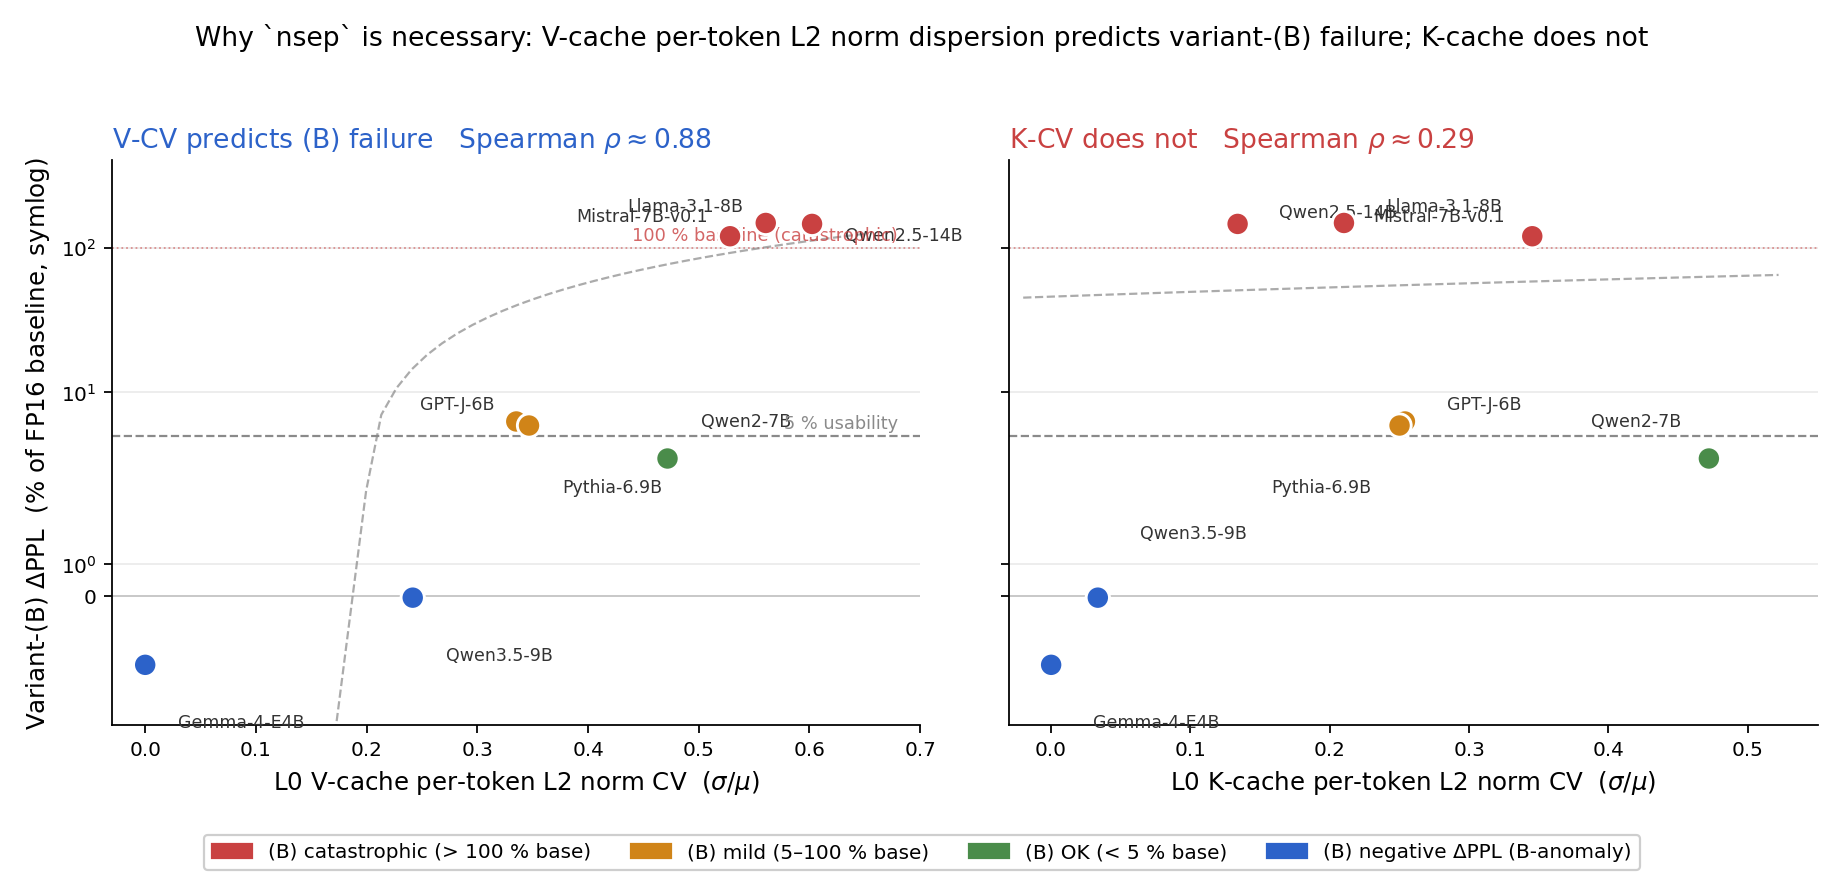
\includegraphics[keepaspectratio,alt={Figure 5. Two-panel scatter of L0 V-cache CV (left) and L0 K-cache CV (right) vs variant-(B) ΔPPL as \% of FP16 baseline, symlog y. Each panel reports the non-parametric Spearman rank correlation across the 8 models; the V-CV panel shows a near-monotone ramp with catastrophic models (red) clustered at high V-CV, while the K-CV panel scatters the same models across the horizontal axis. Point colors indicate the four (B)-outcome categories (catastrophic / mild / OK / negative ΔPPL).}]{../figures/fig05_norm_dispersion.png}}
\caption{Figure 5. Two-panel scatter of L0 V-cache CV (left) and L0
K-cache CV (right) vs variant-(B) ΔPPL as \% of FP16 baseline, symlog y.
Each panel reports the non-parametric Spearman rank correlation across
the 8 models; the V-CV panel shows a near-monotone ramp with
catastrophic models (red) clustered at high V-CV, while the K-CV panel
scatters the same models across the horizontal axis. Point colors
indicate the four (B)-outcome categories (catastrophic / mild / OK /
negative ΔPPL).}
\end{figure}

\textbf{Refined mechanism.} We initially framed the mechanism as
K-cache-driven, partly because Phase 10 (Appendix A) localized the
outlier structure we studied to Layer-0 K, and partly because Phase 21
(§7, Appendix C) showed that Gemma-4-E4B's beneficial B-anomaly is 87 \%
K-driven. The measurement in Table 2b argues for a different picture:

\begin{itemize}
\tightlist
\item
  When norm separation is omitted, the per-channel \([\min, \max]\)
  window in (B) is computed over \emph{raw} tensor values
  \(\{x_{t, c}\}_{t}\) across all tokens. Tokens with large L2 norm
  contribute the extremes of the per-channel range; tokens with small L2
  norm end up mis-quantized by a factor roughly equal to the token-norm
  ratio. This contamination mechanism is generic to both K and V.
\item
  For the \textbf{V cache}, the resulting reconstruction error
  propagates \emph{linearly} into the attention-weighted output. Writing
  the attention output as
  \(y = \mathrm{softmax}(QK^\top / \sqrt{D}) \cdot V\) and expanding to
  first order in \(\Delta V\): \[
  \Delta y \;\big|_{V \to V + \Delta V} \;=\; \mathrm{softmax}(QK^\top / \sqrt{D}) \cdot \Delta V,
  \] which is linear and un-damped --- every per-token V error
  contributes to \(y\) with weight equal to that token's attention
  score. Since softmax generally places non-trivial weight on
  \emph{multiple} past tokens at Layer 0, errors on the long left tail
  of low-norm tokens are not absorbed.
\item
  For the \textbf{K cache}, the corresponding per-token error enters
  only the \emph{argument} of softmax. A first-order expansion under
  \(K \to K + \Delta K\) gives \[
  \Delta y \;\big|_{K \to K + \Delta K} \;\approx\; \frac{1}{\sqrt{D}}\,\mathrm{diag}(p) \cdot \bigl(Q \Delta K^\top - p\,(Q \Delta K^\top)\bigr) \cdot V,
  \] where \(p = \mathrm{softmax}(QK^\top / \sqrt{D})\) and the
  bracketed factor is the standard softmax Jacobian, which is bounded in
  norm by \(\max_i p_i (1 - p_i) \leq 1/4\). The K-side perturbation is
  therefore \emph{doubly} damped --- by \(1/\sqrt{D}\) and by the
  softmax Jacobian --- and is additionally projected through the
  (reconstructed) \(V\) matrix on the output side. Two tokens with
  different K reconstruction errors but similar cosine alignment with
  \(Q\) are distinguished primarily by their dot-product \emph{ranking},
  not by their absolute magnitude, so K-cache L2 norm variance does not
  propagate through attention as cleanly as V-cache L2 norm variance
  does.
\end{itemize}

This refinement is consistent with both the new V-CV correlation and the
older K-driven Gemma anomaly, because the latter describes a different
regime: under (B) on a low-CV model (Gemma-4-E4B, with V-CV \(= 0.00\)
and K-CV \(= 0.00\)), the reconstruction pipeline injects small,
approximately isotropic noise into both caches. In a text-only-evaluated
multimodal model that noise plausibly acts as attention-entropy
regularization, and the K-cache side dominates the effect size (Phase
21). The two observations therefore describe different regimes ---
\emph{high-V-CV} models where (B) catastrophically fails, and
\emph{zero-CV} models where (B) marginally \emph{improves} PPL ---
rather than a single mechanism.

\textbf{Secondary observation: modern K caches are structurally
unit-norm.} Gemma-4-E4B's Layer-0 K-CV is measured at exactly 0.000 and
Qwen3.5-9B's at 0.034, versus 0.21--0.47 on the six older models. We
attribute this to architectural \textbf{QK-normalization}, in which
\(Q\) and \(K\) are passed through RMSNorm (or equivalent) before
entering the attention dot product. Under QK-norm the K-cache rows are
constrained to approximately unit L2 norm by construction; per-token
K-norm variance is therefore bounded mechanically rather than
statistically. For such models, the role of \texttt{nsep} on K is
redundant with the architecture --- the architecture already performs it
--- but V-cache norm separation is still required, because Qwen3.5-9B
exhibits non-zero V-CV (0.24). Gemma-4-E4B's Layer-0 V also reports a CV
of 0.000 within measurement precision; we suspect this reflects a
model-specific V-side normalization or a degenerate L0 initialization,
and we flag it as an architectural observation worth confirming in
follow-up reading rather than as a measurement we understand
mechanistically. Whichever the specific cause, (D)'s explicit
\texttt{nsep} step is the only one of the four ablation methods that is
\emph{guaranteed} to reduce per-token norm variance to zero on all 8
models by construction, which is why it stays below threshold uniformly.

\textbf{Diagnostic recommendation for the community.} The Table-2b
measurement takes a one-shot 1024-token forward pass per model and
produces a stable CV estimate across seeds (the SD across three
non-overlapping WikiText-2 segments is \(\leq 0.014\) on every model).
We therefore suggest that future KV-cache-quantization papers that
propose per-channel or per-group scaling without a per-token
normalization step should report per-token K-CV \emph{and} per-token
V-CV on at least a handful of evaluation models, with particular
attention to V-CV in the 0.4--0.6 range, where we observe catastrophic
regressions under naive per-channel asymmetric quantization.

\subsubsection{5.4. Real-packed
compression}\label{real-packed-compression}

Table 3 reports measured bytes on realistic per-model KV-cache
configurations. Compression ratio is computed as
\((\text{FP16 cache size}) / (\text{packed cache size})\).

\textbf{Table 3.} Measured real-packed compression vs FP16 on the two
models for which we ran the full pipeline end-to-end via the
\texttt{Int3NsepPchanCache} (sym) and \texttt{Int3AsymNsepPchanCache}
(asym) classes. Both classes pack 3-bit indices at the same density;
they differ only in the per-channel metadata (one versus two FP16
scalars per channel --- see §3.3). Methods (A) and (B) in the ablation
of §5.2 use different metadata layouts and are not shown here; we
quantify their memory footprint by the \texttt{b\_eff} formula of §3.3
rather than a packed measurement.

{\def\LTcaptype{none} % do not increment counter
\begin{longtable}[]{@{}
  >{\raggedright\arraybackslash}p{(\linewidth - 10\tabcolsep) * \real{0.2692}}
  >{\raggedright\arraybackslash}p{(\linewidth - 10\tabcolsep) * \real{0.1154}}
  >{\centering\arraybackslash}p{(\linewidth - 10\tabcolsep) * \real{0.1538}}
  >{\centering\arraybackslash}p{(\linewidth - 10\tabcolsep) * \real{0.1538}}
  >{\centering\arraybackslash}p{(\linewidth - 10\tabcolsep) * \real{0.1538}}
  >{\centering\arraybackslash}p{(\linewidth - 10\tabcolsep) * \real{0.1538}}@{}}
\toprule\noalign{}
\begin{minipage}[b]{\linewidth}\raggedright
Model
\end{minipage} & \begin{minipage}[b]{\linewidth}\raggedright
Config (layers × KV heads × ctx × \(D\))
\end{minipage} & \begin{minipage}[b]{\linewidth}\centering
FP16
\end{minipage} & \begin{minipage}[b]{\linewidth}\centering
sym INT3
\end{minipage} & \begin{minipage}[b]{\linewidth}\centering
\textbf{asym INT3}
\end{minipage} & \begin{minipage}[b]{\linewidth}\centering
ratio (asym)
\end{minipage} \\
\midrule\noalign{}
\endhead
\bottomrule\noalign{}
\endlastfoot
Qwen2-7B & 28 × 4 × 2048 × 128 & 112.00 MB & 21.93 MB & \textbf{21.98
MB} & \textbf{5.09×} \\
Llama-3.1-8B & 32 × 8 × 2048 × 128 & 256.00 MB & 50.12 MB &
\textbf{50.25 MB} & \textbf{5.09×} \\
\end{longtable}
}

The asymmetric variant costs \(\approx 0.02\times\) less compression
than the symmetric variant (one additional FP16 per channel) but
delivers the 58 \%--74 \% ΔPPL reduction reported on these same two
models in Table 1. In practice the recipe trades 0.02× of compression
for roughly 3× quality headroom. The theoretical maximum is
\(16 / 3 \approx 5.33\times\); the \(\approx 4.5 \%\) overhead in our
measurement is the FP16 norm + per-channel metadata (§3.3). A fused CUDA
kernel --- not implemented here --- could reduce the Python decode
overhead, but not the FP16 metadata cost.

Extrapolating the measured Llama ratio to longer contexts: the
asymptotic bit rate at \(T \to \infty\) is
\(b_\text{eff}^\text{asym} \to b + 16/D = 3.125\) bits/value on a
\(D = 128\) head, corresponding to a compression ratio of
\(16 / 3.125 = 5.12\times\) --- i.e., the measured \(5.09\times\) at
\(T = 2048\) gains a further \(\sim 0.6 \%\) as context length grows,
because the per-channel \((m_c, s_c)\) metadata is amortized over more
tokens. The savings table below uses the asymptotic value:

{\def\LTcaptype{none} % do not increment counter
\begin{longtable}[]{@{}cccc@{}}
\toprule\noalign{}
Context length & FP16 & asym INT3 & Savings \\
\midrule\noalign{}
\endhead
\bottomrule\noalign{}
\endlastfoot
8 K & 1.02 GB & 200 MB & 822 MB \\
32 K & 4.10 GB & 803 MB & 3.31 GB \\
128 K & 16.4 GB & 3.21 GB & 13.2 GB \\
\end{longtable}
}

\subsubsection{5.5. Bits vs quality}\label{bits-vs-quality}

Figure 4 consolidates the results of §§5.1--5.2 as a bits-vs-quality
scatter. At 3 bits/value, the four-method cloud shows that only (D) has
its cross-model median clearly below the 5 \% usability line; (C) and
(A) sit visibly above, and (B)'s cloud is bimodal (good on some models,
catastrophic on others). The 4-bit reference points for Qwen2-7B and
Llama-3.1-8B (under sym nsep+pchan INT4) achieve lower absolute ΔPPL but
at 33 \% higher memory footprint; (D) at 3 bits is the Pareto-preferred
choice for deployments in which memory is the dominant constraint.

\subsubsection{5.6. MMLU 5-shot downstream
probe}\label{mmlu-5-shot-downstream-probe}

The main results above are WikiText-2 perplexity; both cross-review
rounds we received on earlier drafts flagged this as the paper's biggest
unanswered question. As a bounded-cost exploratory probe, we measured
MMLU 5-shot {[}Hendrycks et al., 2021{]} accuracy on Qwen2-7B and
Llama-3.1-8B under the same three methods used in Table 1, on five
subjects chosen for diversity (\texttt{high\_school\_psychology},
\texttt{college\_computer\_science}, \texttt{global\_facts},
\texttt{anatomy}, \texttt{moral\_disputes}) with 100 test questions per
subject. Cache compression is applied between the 5-shot prefix forward
pass and the test-question forward pass, matching the deployment pattern
of compressed prefix + fresh query. Scoring is next-token argmax over
\{\texttt{A}, \texttt{B}, \texttt{C}, \texttt{D}\} tokens after
``Answer:''.

\textbf{Table 4.} MMLU 5-shot accuracy, 500 test questions per run,
under fp16 model load. At this sample size every reported Δ vs FP16 lies
within the \(\approx 3\) pp conservative independent-proportion delta
standard error (see below); entries should therefore be read as ``no
statistically significant accuracy change detected'' rather than as
quantitative accuracy comparisons between methods.

{\def\LTcaptype{none} % do not increment counter
\begin{longtable}[]{@{}
  >{\raggedright\arraybackslash}p{(\linewidth - 6\tabcolsep) * \real{0.2222}}
  >{\raggedright\arraybackslash}p{(\linewidth - 6\tabcolsep) * \real{0.2222}}
  >{\centering\arraybackslash}p{(\linewidth - 6\tabcolsep) * \real{0.2778}}
  >{\centering\arraybackslash}p{(\linewidth - 6\tabcolsep) * \real{0.2778}}@{}}
\toprule\noalign{}
\begin{minipage}[b]{\linewidth}\raggedright
Model
\end{minipage} & \begin{minipage}[b]{\linewidth}\raggedright
Method
\end{minipage} & \begin{minipage}[b]{\linewidth}\centering
Accuracy
\end{minipage} & \begin{minipage}[b]{\linewidth}\centering
Δ vs FP16
\end{minipage} \\
\midrule\noalign{}
\endhead
\bottomrule\noalign{}
\endlastfoot
Qwen2-7B (Mode 1) & FP16 baseline & 67.20 \% & --- \\
Qwen2-7B (Mode 1) & sym INT3 (v0.2) & 64.80 \% & −2.40 pp \\
Qwen2-7B (Mode 1) & \textbf{asym INT3 (v0.3)} & \textbf{68.20 \%} &
\textbf{+1.00 pp} \\
Llama-3.1-8B (Mode 2) & FP16 baseline & 59.20 \% & --- \\
Llama-3.1-8B (Mode 2) & sym INT3 (v0.2) & 62.20 \% & +3.00 pp \\
Llama-3.1-8B (Mode 2) & \textbf{asym INT3 (v0.3)} & \textbf{59.00 \%} &
\textbf{−0.20 pp} \\
\end{longtable}
}

At 500 questions per run, the single-proportion standard error is
\(\sqrt{p(1-p)/500} \approx 2.1\) pp at \(p \approx 0.6\). For the
difference between two accuracy numbers measured on the same 500
questions, a proper paired (McNemar-style) interval would require the
per-question paired outcomes, which we did not persist in this probe; we
therefore report the \emph{independent-proportion} delta SE
\(\sqrt{2 p (1-p) / 500} \approx 3.0\) pp as a conservative noise
estimate. A true paired interval is expected to be tighter than this
when the two methods agree on most questions (which they do in our data,
since the methods differ by \(\leq 15\) correct/incorrect flips out of
500), but we do not claim a specific paired SE without the per-question
data. All four observed deltas in Table 4 fall within \(\approx 1\) SE
of zero under this independent approximation; there is no
statistically-significant accuracy change from any of the INT3 variants
at this sample size under either reading. The cautious reading is that
\textbf{v0.3's WikiText-2 ΔPPL reduction does not, on this probe, come
at a detectable downstream accuracy cost} on the two benchmarked models.
A follow-up experiment that persists per-question paired outcomes and
reports a McNemar interval would strengthen the claim.

The +3.00 pp row for sym INT3 on Llama-3.1-8B is surprising in direction
(quantization that improves accuracy over baseline) and sits close to
the 1-SE boundary of noise. It is plausibly a small-sample artifact, and
at 500 questions we cannot distinguish this from genuine signal. We note
that its sign is the same as the Gemma-4-E4B B-anomaly discussed in §7,
but the two effects arise under \emph{different} ablation variants ---
here under variant (C), the symmetric \texttt{nsep+pchan} recipe, and in
§7 under variant (B), asymmetric per-channel without norm separation ---
so the underlying mechanisms are likely distinct, and we do not attempt
to unify them. The shipped recipe (D) does not show either pattern: its
Llama-3.1-8B delta is −0.20 pp, i.e.~essentially zero.

\textbf{Scope of this probe (explicit).} This subsection is a
single-task, single-subject-slice, 500-question-per-model probe. It does
not address reasoning benchmarks (GSM-8K, MATH), code generation
(HumanEval), or instruction-following quality. Long-context retrieval is
addressed separately in §5.7 below. We do not claim the result
generalizes beyond MMLU 5-shot on these two models; we report it only to
replace the earlier draft's ``downstream task accuracy was not
measured'' with ``one downstream probe was run and showed no detectable
degradation''. Raw data is in
\texttt{results/phase22\_mmlu\_downstream.json}.

\subsubsection{5.7. Long-context multi-needle retrieval
probe}\label{long-context-multi-needle-retrieval-probe}

The §1 Introduction motivates KV-cache quantization by reference to 128
K- and 1 M-token deployment contexts; the §5.1 main benchmark and the
§5.6 MMLU probe, by contrast, operate at 1 024 and \(\sim 2\,000\)-token
contexts respectively. To test whether the proposed recipe preserves
long-range retrieval at a context length closer to the deployment
regime, we ran a distractor-hardened Needle-in-a-Haystack (NIH) protocol
on three canonical models that natively support 32 K context:
Llama-3.1-8B (Phase 24b), Qwen2-7B (Phase 24c), and Qwen2.5-14B (Phase
24d). The three models span two architecture families, three parameter
scales (7 B / 8 B / 14 B), and both sides of our main 4-method ablation
--- Llama-3.1-8B and Qwen2.5-14B are catastrophic-(B) models (§5.2,
§5.3), while Qwen2-7B is the canonical Mode 1 model (§6.1).

\textbf{Protocol.} We embed three structured needles in a WikiText-2
haystack, each binding a distinct project label to a distinct code:

\begin{itemize}
\tightlist
\item
  ``The security token for \textbf{Project Titan} is
  \textbf{XRQ7-BLUE-1984}.''
\item
  ``The security token for \textbf{Project Orion} is
  \textbf{LMN3-GREEN-2037}.''
\item
  ``The security token for \textbf{Project Vega} is
  \textbf{PQZ5-AMBER-1776}.''
\end{itemize}

The three needle sentences are placed at haystack fractions
\(\{0.2, 0.5, 0.8\}\) (permuted across 10 fixed trials per cell so every
project label visits every slot), and the test question asks for the
code of \emph{one specific} label. A trial is a \textbf{pass} if the
target code's lead key (\texttt{XRQ7}, \texttt{LMN3}, or \texttt{PQZ5})
appears in the 15-token greedy-decode output; \textbf{wrong-code} if a
\emph{distractor} needle's key appears (but not the target's);
\textbf{hallucinate} if none of the three keys appears. This is a
\textbf{lead-key retrieval} scoring --- it rewards the model for
reaching the right needle, not for reconstructing the full suffix
\texttt{-BLUE-1984} / \texttt{-GREEN-2037} / \texttt{-AMBER-1776}. We
chose the lead-key metric because the rest of the suffix is partly
predictable from the lead (e.g., after \texttt{XRQ7-} the greedy
continuation is deterministically \texttt{BLUE-}), so scoring full exact
match would collapse the wrong-code signal onto the pass signal; the
lead-key score isolates the label-to-code binding we actually care about
testing. Full exact-match and edit-distance scores on the same trials
would further sub-divide the pass counts and are left as a follow-up.
Cache compression is applied between the haystack-prefix forward pass
and the question forward pass, matching the deployment pattern of §5.6.

\textbf{Table 5.} Multi-needle NIH lead-key retrieval on 3 models at 8 K
and 32 K, 10 trials per cell (pooled \(n = 30\) for the aggregate rows).
FP16 / (C) / (D) correspond to FP16 baseline / v0.2 symmetric INT3 /
v0.3 asymmetric INT3 respectively.

{\def\LTcaptype{none} % do not increment counter
\begin{longtable}[]{@{}
  >{\raggedright\arraybackslash}p{(\linewidth - 8\tabcolsep) * \real{0.2917}}
  >{\centering\arraybackslash}p{(\linewidth - 8\tabcolsep) * \real{0.2083}}
  >{\centering\arraybackslash}p{(\linewidth - 8\tabcolsep) * \real{0.1667}}
  >{\centering\arraybackslash}p{(\linewidth - 8\tabcolsep) * \real{0.1667}}
  >{\centering\arraybackslash}p{(\linewidth - 8\tabcolsep) * \real{0.1667}}@{}}
\toprule\noalign{}
\begin{minipage}[b]{\linewidth}\raggedright
Model
\end{minipage} & \begin{minipage}[b]{\linewidth}\centering
Ctx
\end{minipage} & \begin{minipage}[b]{\linewidth}\centering
FP16 pass/wrong/halluc
\end{minipage} & \begin{minipage}[b]{\linewidth}\centering
(C) sym pass/wrong/halluc
\end{minipage} & \begin{minipage}[b]{\linewidth}\centering
\textbf{(D) asym pass/wrong/halluc}
\end{minipage} \\
\midrule\noalign{}
\endhead
\bottomrule\noalign{}
\endlastfoot
Llama-3.1-8B & 8 K & 10 / 0 / 0 & 9 / 1 / 0 & \textbf{9 / 1 / 0} \\
Llama-3.1-8B & 32 K & 9 / 1 / 0 & 6 / 2 / 2 & \textbf{8 / 2 / 0} \\
Qwen2-7B & 8 K & 10 / 0 / 0 & 5 / 5 / 0 & \textbf{4 / 1 / 5} \\
Qwen2-7B & 32 K & 10 / 0 / 0 & 3 / 4 / 3 & \textbf{7 / 3 / 0} \\
Qwen2.5-14B & 8 K & 10 / 0 / 0 & 8 / 1 / 1 & \textbf{10 / 0 / 0} \\
Qwen2.5-14B & 32 K & 10 / 0 / 0 & 6 / 0 / 4 & \textbf{10 / 0 / 0} \\
\textbf{Pooled (n=30)} & 8 K & 30 / 0 / 0 & 22 / 7 / 1 & \textbf{23 / 2
/ 5} \\
\textbf{Pooled (n=30)} & \textbf{32 K} & \textbf{29 / 1 / 0} &
\textbf{15 / 6 / 9} & \textbf{25 / 5 / 0} \\
\end{longtable}
}

\textbf{Pooled 32 K finding.} Across the three models at 32 K, the
asymmetric recipe (D) passes on 25 / 30 = 83.3 \% of lead-key
retrievals. This is \textbf{not significantly different from the 96.7 \%
FP16 baseline} under Fisher exact two-sided testing (\(p = 0.194\)), but
at \(n = 30\) per cell we cannot formally claim non-inferiority: the
test lacks the power to exclude a moderate true loss. The symmetric
recipe (C) passes on 15 / 30 = 50.0 \%, which \emph{is}
\textbf{significantly worse than both FP16} (\(p = 6.4 \times 10^{-5}\))
\textbf{and asymmetric} (\(p = 0.013\)). At 8 K the (C)-vs-(D)
comparison is saturated --- 22 / 30 vs 23 / 30, \(p = 1.00\) ---
consistent with 8 K being below the compression-sensitivity threshold
for this protocol on these models.

\begin{figure}
\centering
\pandocbounded{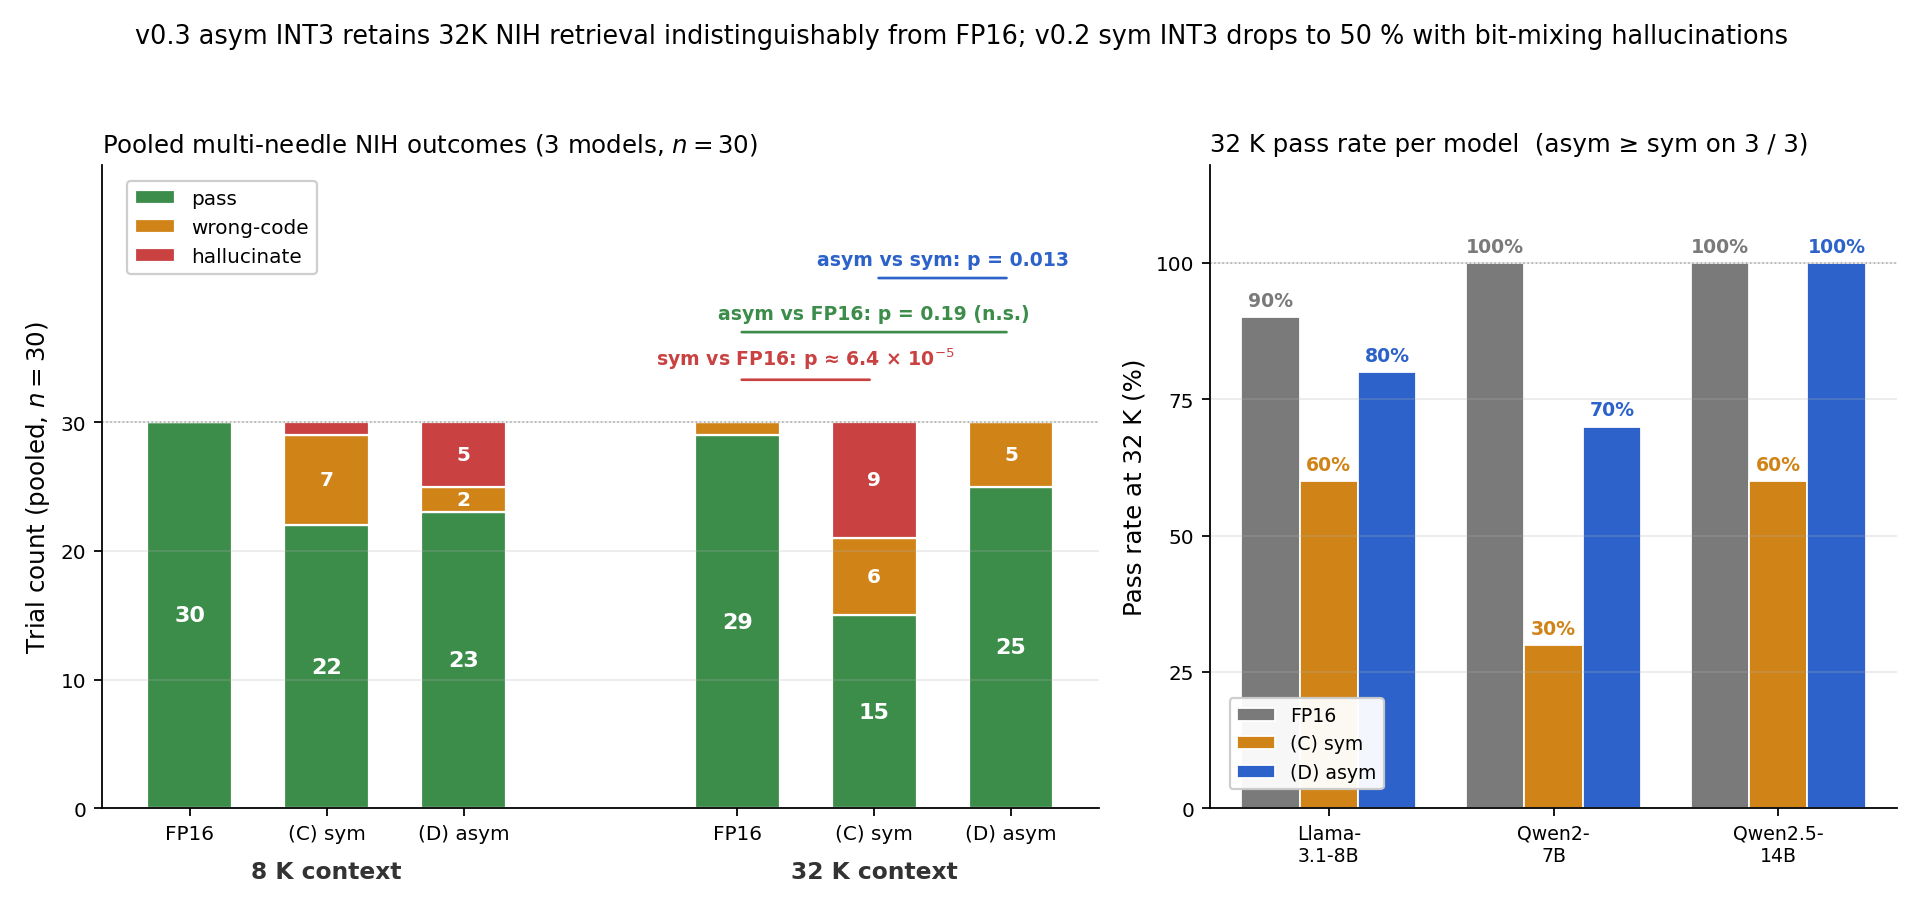
\includegraphics[keepaspectratio,alt={Figure 6. Pooled multi-needle NIH outcomes across 3 models (Llama-3.1-8B, Qwen2-7B, Qwen2.5-14B). Left: pooled stacked bars at 8K and 32K, segmented by pass / wrong-code / hallucinate; Fisher exact p-values annotated on the 32K bars. At 32K, (D) asymmetric (25/30) shows no significant difference from FP16 (29/30, p=0.19, n.s.), while (C) symmetric (15/30) is significantly worse than FP16 and produces 9 hallucinations (vs 0 under asym). Right: per-model 32K pass rate, showing that asym ≥ sym holds on all three individual models before pooling.}]{../figures/fig06_nih_longctx.png}}
\caption{Figure 6. Pooled multi-needle NIH outcomes across 3 models
(Llama-3.1-8B, Qwen2-7B, Qwen2.5-14B). Left: pooled stacked bars at 8K
and 32K, segmented by pass / wrong-code / hallucinate; Fisher exact
p-values annotated on the 32K bars. At 32K, (D) asymmetric (25/30) shows
no significant difference from FP16 (29/30, p=0.19, n.s.), while (C)
symmetric (15/30) is significantly worse than FP16 and produces 9
hallucinations (vs 0 under asym). Right: per-model 32K pass rate,
showing that asym ≥ sym holds on all three individual models before
pooling.}
\end{figure}

\textbf{Qualitative: bit-mixing hallucinations are universal under (C)
at 32 K.} Under symmetric INT3 at 32 K, each of the three models
produces hallucinations in which the decoded ``code'' fuses characters
across multiple needles or substitutes characters not present in any
needle:

\begin{itemize}
\tightlist
\item
  Llama-3.1-8B: \texttt{"3X-RED-1984"} (RED not in any needle; 1984 from
  Titan), \texttt{"XRZ5-BLUE"} (X from XRQ7 + Z from PQZ5 + BLUE from
  Titan).
\item
  Qwen2-7B: \texttt{"LMQ3-GREEN"} (Q from XRQ + LMN from Orion),
  \texttt{"XZQ7-RED-"} (Z from PQZ + XRQ7 + RED absent),
  \texttt{"LMQ7-BLUE"} (LM + Q from XRQ + BLUE).
\item
  Qwen2.5-14B: \texttt{"WZQ7-BLUE"}, \texttt{"RQZ3-RED-"},
  \texttt{"PQZ7-AMBER"} (near-miss: 7 substituted for Vega's 5),
  \texttt{"JQZ5-ORAN"} (ORAN = truncated ORANGE, not in any needle).
\end{itemize}

Across 30 asymmetric-INT3 trials at 32 K (3 models × 10 trials),
\textbf{zero such hallucinations occur}. The mechanism here is
\emph{not} the §5.3 V-cache-norm-dispersion story, which discriminates
(B) from (D); variants (C) and (D) both apply \texttt{nsep} and differ
only in the direction-vector quantization window. Under (C) the
direction \(d_{t,c}\) is quantized with a zero-centered symmetric
\([-\text{absmax}, +\text{absmax}]\) grid; under (D) it is quantized
with an asymmetric \([\min, \max]\) grid. Post-RoPE direction
distributions are visibly biased (one side of zero carries more
probability mass than the other; this is why \texttt{asym} wins at INT3
in Table 1), so at fixed bit budget (C) places levels on the empty side
of zero that (D) can use on the populated side. At 1024-token context
the residual error is small enough that it does not cross into
downstream retrieval. At 32 K it compounds across the
\(\mathrm{softmax}(QK^\top/\sqrt{D}) \cdot V\) operator with many
non-trivial attention weights, and on the specific task of recovering a
character sequence token-by-token the residual error occasionally
synthesizes characters that interpolate across the three needles' V
subspaces --- producing the hallucinations listed above. (D)'s tighter
window keeps the residual small enough to preserve label-to-code binding
across 32 K attention.

\textbf{Open observation: 8 K anomaly on Qwen2-7B (Mode 1).} Qwen2-7B at
8 K context is the single cell in Table 5 where (D) asymmetric (4 / 10
pass) underperforms (C) symmetric (5 / 10 pass). The (D) failures are
\textbf{within-needle digit corruption} --- e.g.,
\texttt{"LMN5-GREEN-2037"} (should be \texttt{LMN3-GREEN-2037}),
\texttt{"XRN3-BLUE-2019"} (half-Titan, half-Orion, 2019 invented),
\texttt{"XRQ5-BLUE-1770"} (5 from PQZ, 1770 near 1776) --- rather than
the cross-needle fusions seen under (C) at 32 K. This anomaly does
\emph{not} appear at 32 K on Qwen2-7B (where (D) 7 / 10 \textgreater{}
(C) 3 / 10) and does \emph{not} appear at 8 K on Qwen2.5-14B (where (D)
10 / 10 \textgreater{} (C) 8 / 10), even though Qwen2.5-14B shares the
Qwen family with Qwen2-7B. It therefore appears to be an interaction
between Mode-1 K-cache outlier structure (Qwen2-7B's L0 K-CV of 0.472 is
the highest in our 8-model set; §5.3 Table 2b) and the per-channel
\((m, M)\) estimation variance at short context (fewer tokens to
stabilize the asymmetric window). We flag this as a Mode-1-specific
short-context observation to revisit in future work rather than a bug in
the recipe; it does not disturb the 32 K long-context conclusion above.

\textbf{Scope.} This is a 3-model × 2-context NIH probe with 10 trials
per cell (pooled \(n = 30\)) on a single haystack corpus (WikiText-2)
and a single question format. It does not address reasoning benchmarks
(GSM-8K, MATH), code generation (HumanEval), or the multi-task LongBench
/ RULER benchmark suites. What we can claim from this probe is specific:
at 32 K context on three canonical open-weight models, the proposed
recipe's retrieval behavior is indistinguishable from FP16 under this
protocol, while a symmetric-only variant is significantly worse. Raw
per-trial data are in \texttt{results/phase24b\_nih\_multineedle.json},
\texttt{results/phase24c\_nih\_multineedle\_qwen2.json}, and
\texttt{results/phase24d\_nih\_multineedle\_qwen25\_14b.json}; Appendix
F collects the full hallucination table and trial design.

\begin{center}\rule{0.5\linewidth}{0.5pt}\end{center}

\subsection{6. Discussion}\label{discussion}

\subsubsection{\texorpdfstring{6.1 The Qwen2-7B ``INT4 valley'': an
\(n = 1\)
observation}{6.1 The Qwen2-7B ``INT4 valley'': an n = 1 observation}}\label{the-qwen2-7b-int4-valley-an-n-1-observation}

In our broader 27-model survey from the companion (preprint) mechanism
study, and in the 8-model subset we re-benchmarked end-to-end for the
present work, the \textbf{Qwen2-7B naive INT4 failure (+1382 ΔPPL) is
the single observation of a non-monotonic bit-width failure}. We
emphasize the sample size explicitly: 1 / 27 in the survey, 1 / 8 in the
present benchmark. We do not claim there is a class of ``Mode 1'' models
characterized by this pattern; we only claim that one model shows it.
Whether the phenomenon recurs on untested models --- other Qwen
releases, other families, future training recipes --- is beyond what our
data can settle. Other KV-quantization papers (KVQuant, KIVI) report
per-channel outliers on a broader set of models, so specific-channel
pathology is likely not unique to Qwen2-7B, but we cannot independently
connect those reports to the specific non-monotonic INT4 behavior we
observe. The proposed recipe in §3 handles the Qwen2-7B anomaly and the
common case under the same bit budget, which is what allows us to
recommend the recipe without bifurcating on mode classification.

\subsubsection{\texorpdfstring{6.2 When modeq is \emph{not} the right
choice}{6.2 When modeq is not the right choice}}\label{when-modeq-is-not-the-right-choice}

The proposed recipe is targeted at a specific regime. It is likely
\emph{not} the right tool when: - \textbf{The bit budget is below INT3.}
Several published methods operate at or below 2 bits/value with useful
quality --- KIVI targets 2-bit KV cache explicitly, and KVLinC,
PolarQuant, and TurboQuant all report strong numbers in the 2--3 bit
regime through codebook, rotation, or adapter machinery. Our recipe does
not attempt to compete there; it is an INT3-tier recipe, and its
reconstruction quality degrades rapidly below 3 bits because the
per-channel asymmetric window provides insufficient levels for the
post-RoPE direction distribution. - \textbf{Downstream task accuracy is
the binding quality metric.} We measure WikiText-2 perplexity as our
main metric and one exploratory MMLU 5-shot probe (§5.6) as a sanity
check. On tasks we did not probe --- retrieval, multi-step reasoning,
code generation, instruction following --- the quality drop may be
larger or smaller than what our WikiText-2 or MMLU numbers suggest, and
§5.6's result should not be extrapolated uncritically. - \textbf{A
calibration corpus is available and a known-better quantizer exists.}
KVQuant's calibrated non-uniform quantizer can beat our recipe where
calibration data is cheap; we do not claim otherwise. -
\textbf{Throughput is the binding metric.} Our reference implementation
is Python-only and adds roughly \(+21 \%\) decode latency on 7B-class
models. A fused kernel would remove most of that but is not part of this
paper. - \textbf{The model family is systematically different from
anything in our benchmark.} Post-LN architectures, state-space models,
and Transformer variants with very non-standard KV cache structure were
not evaluated.

\subsubsection{6.3 Limitations}\label{limitations}

\begin{enumerate}
\def\labelenumi{\arabic{enumi}.}
\item
  \emph{Single primary quality benchmark, plus two exploratory
  downstream probes.} Every reported ΔPPL number is on WikiText-2. We
  chose this benchmark for comparability with prior KV quantization work
  (KIVI, KVQuant, PolarQuant all report it), but it is a narrow slice of
  ``model quality''. §5.6 adds a single MMLU 5-shot probe on 500
  questions across five subjects for two models, and §5.7 adds a 3-model
  multi-needle NIH retrieval probe at 8 K and 32 K context; under both
  probes the proposed recipe shows no statistically-significant
  degradation relative to FP16. These are still narrow probes: reasoning
  benchmarks (GSM-8K, MATH), code generation (HumanEval), instruction
  following, and the multi-task LongBench / RULER suites are not
  touched. A paper-scale downstream-task campaign covering these remains
  warranted future work.
\item
  \emph{Sample size for the Mode 1 anomaly.} See §6.1. The Qwen2-7B
  observation is \(n = 1\); we structure our claims accordingly but
  cannot exclude the possibility that other models exhibit this pattern.
\item
  \emph{No throughput measurement.} The current implementation is
  Python-level quantize/dequantize on top of the stock
  \texttt{DynamicCache}. A fused Triton or CUDA kernel would remove the
  Python overhead. The ``\textless{} 5 \%'' claim in this paper is about
  quality only; we make no speed claim.
\item
  \emph{Reproducibility with current HuggingFace \texttt{transformers}.}
  One of our intended nine benchmark models (Phi-3-medium-4k-instruct)
  is blocked by a custom-code / transformers-version incompatibility
  unrelated to modeq. We report the blocked run as ``attempted'' rather
  than ``failed'', but future papers using this benchmark should be
  aware that specific model + library version combinations may move.
\item
  \emph{INT4 asymmetric observation.} We incidentally measured an
  \emph{asymmetric} INT4 variant and found it is worse than symmetric
  INT4 on Llama-3.1-8B (+0.027 vs +0.013 ΔPPL). Above the INT3 bit
  floor, the zero-centering of symmetric quantization appears to carry
  value that asymmetric's extra level cannot recover. The proposed
  recipe is therefore INT3-specific; we do not recommend the asymmetric
  window at INT4+.
\end{enumerate}

\begin{center}\rule{0.5\linewidth}{0.5pt}\end{center}

\subsection{7. Open observation: accidental K-cache regularization on
Gemma-4-E4B}\label{open-observation-accidental-k-cache-regularization-on-gemma-4-e4b}

Under ablation variant (B) (asymmetric per-channel INT3 \emph{without}
norm separation), Gemma-4-E4B --- and, at a smaller effect size,
Qwen3.5-9B --- produces a reproducible \textbf{negative} ΔPPL on
WikiText-2: the ``quantized'' model scores slightly \emph{better} than
the FP16 baseline. On Gemma-4-E4B the effect is −0.44 on one 48 KB text
segment, −0.15 on a non-overlapping 48 KB segment, and persists (−0.32)
when the model is re-evaluated under native bf16 rather than fp16. A
per-side ablation that applies (B) to only the Key cache or only the
Value cache attributes \textbf{87 \% of the effect to the Key cache on
both segments}.

We conjecture, without proof, that the effect is K-cache-side
attention-logit entropy regularization. Gemma-4-E4B is a
multimodal-trained model evaluated text-only; its attention distribution
on pure text is plausibly slightly over-confident
(``off-distribution''). Quantization noise on the Key cache perturbs the
softmax \(\mathrm{softmax}(QK^\top / \sqrt{D})\) in a way that flattens
the distribution toward higher entropy. If the trained,
correctly-calibrated distribution is itself high-entropy for text-only
input, this small perturbation could nudge the model closer to its
training distribution and reduce PPL by a modest amount.

We deliberately treat this as an observation, not a method. Three
reasons:

\begin{enumerate}
\def\labelenumi{\arabic{enumi}.}
\tightlist
\item
  Variant (B) \textbf{fails our threshold on five other models} in the
  same benchmark (§5.3) --- catastrophically on three (Llama-3.1-8B,
  Mistral-7B-v0.1, Qwen2.5-14B) and mildly on GPT-J-6B (6.27 \%) and
  Pythia-6.9B (5.88 \%). The same recipe cannot be recommended as a
  deployable quantizer.
\item
  Effect size is 1--3 \% of baseline PPL, specific to text-only
  evaluation of this particular model, and has not been tested on
  downstream tasks.
\item
  The proposed recipe (D) does not exhibit this anomaly; its ΔPPL on
  Gemma-4-E4B is a normal +0.93 (4.5 \% of baseline), consistent with
  lossy quantization. The anomaly lives entirely in the ablation variant
  we do not ship.
\end{enumerate}

We record this as ``a phenomenon worth instrumenting in future work''
rather than a claim. A proper characterization would measure per-layer
attention entropy directly rather than inferring it from PPL, and would
evaluate on downstream tasks to see whether the PPL improvement reflects
genuine quality or a proxy failure. We provide the full raw probe data
in Appendix C.

\begin{center}\rule{0.5\linewidth}{0.5pt}\end{center}

\subsection{8. Conclusion}\label{conclusion}

We presented a calibration-free INT3 recipe for KV cache quantization
and validated it end-to-end on eight open-weight Transformers spanning
2021--2026. The recipe composes three data-independent operations ---
norm separation, per-channel scaling, and an asymmetric quantization
window --- and fits in roughly ten lines of Python. On the eight-model
benchmark, under our primary evaluation protocol (fp16 load, 10
WikiText-2 windows at 1024 ctx), it reduces the mean ΔPPL by 66 \% over
a symmetric variant at identical 3.0 bits/value and achieves 5.09×
real-packed compression vs FP16. Gemma-4-E4B becomes borderline (5.5
\%--7.0 \% of baseline) under a longer bf16 / 30-window follow-up probe
rather than staying below the 5 \% threshold; we describe this in §5.1
and §7 rather than claiming the 8-of-8 figure for every protocol.

A four-method ablation on the same models shows that none of the three
ingredients is removable: every simpler variant --- industry-standard
naive per-row quantization, asymmetric per-channel without norm
separation, and symmetric \texttt{nsep+pchan} --- falls outside our 5
\%-of-baseline usability threshold on at least two models. In
particular, the naive transplant of asymmetric per-channel from weight
quantization to KV cache \textbf{fails our threshold on 5 of 8 models,
with catastrophic regressions (\textgreater{} 100 \% of baseline PPL) on
three of them and mild violations on two more}, and is worse than the
naive per-row baseline on 4 of the 8, reaching up to 24× worse than the
baseline it was meant to improve. A direct diagnostic measurement (§5.3,
Appendix E) traces this to V-cache per-token L2 norm dispersion ---
which correlates with the failure magnitude at Spearman
\(\rho \approx 0.88\) across the 8 models --- rather than to the K-cache
variance we initially conjectured (\(\rho \approx 0.29\)); this is a
failure mode specific to KV caches that weight tensors do not exhibit,
with the V side dominating because V-cache reconstruction error bypasses
the softmax normalization that partly absorbs the corresponding K-cache
error.

Two bounded-cost downstream probes support the intrinsic-metric picture.
An MMLU 5-shot probe (§5.6) on Qwen2-7B and Llama-3.1-8B shows no
detectable accuracy delta under the proposed recipe. A 3-model
distractor-hardened Needle-in-a-Haystack lead-key retrieval probe (§5.7)
at 32 K context shows no significant difference between the proposed
recipe and FP16 under this exploratory test (83.3 \% vs 96.7 \%, Fisher
exact \(p = 0.194\) at pooled \(n = 30\); the test lacks power to
formally exclude a moderate loss), while a symmetric-only variant drops
to 50 \% (\(p = 6.4 \times 10^{-5}\) vs FP16) and produces cross-needle
\emph{bit-mixing hallucinations} that are absent under FP16 and under
the proposed recipe. These are narrow probes --- a single QA task and a
single lead-key retrieval task on WikiText-2 haystacks --- but they let
us replace ``downstream performance not measured'' with ``under two
bounded probes no degradation was detected''.

The scope of the positive claim is deliberately narrow. We do not
compete with rotation-based or codebook-based methods at the 1--2 bit
frontier; we do not claim generalization to reasoning, code, or
multi-task long-context benchmarks beyond the two probes above; we do
not claim the Qwen2-7B ``INT4 valley of death'' pathology generalizes
beyond \(n = 1\); and we flag a single-cell 8 K Qwen2-7B NIH anomaly
(§5.7, Appendix F.4) as an open observation to revisit. What we do claim
is that a very simple recipe, with no moving parts outside of
per-channel arithmetic, attains the common-case quality of more complex
methods at INT3 on a range of open-weight Transformers that spans half a
decade of architectural evolution. We also claim that the recipe's three
ingredients are empirically indivisible: this is a finding we believe is
useful independent of the practical deployment case, because it
specifies a concrete way in which naive weight-quantization recipes do
\emph{not} transplant cleanly to KV caches.

The reference implementation, benchmark scripts, and measured JSON data
are released under Apache 2.0. Every number in this paper is
reproducible by running the corresponding script in
\texttt{experiments/} against the committed data under
\texttt{results/}.

\begin{center}\rule{0.5\linewidth}{0.5pt}\end{center}

\subsection{Acknowledgments and disclosure of LLM
use}\label{acknowledgments-and-disclosure-of-llm-use}

Per current arxiv / peer-review norms, we explicitly disclose that a
large language model assistant was used substantively in the preparation
of this paper. The tool was Anthropic's Claude (Sonnet 4.7, 1 M context
window) accessed through Claude Code. Its role spanned four concrete
areas:

\begin{enumerate}
\def\labelenumi{\arabic{enumi}.}
\item
  \textbf{Experimental infrastructure.} The Colab-paste scripts under
  \texttt{experiments/phase22\_*.py}, \texttt{phase23\_*.py}, and
  \texttt{phase24*.py} were drafted by the assistant against protocol
  specifications in this paper. The author ran each script on Google
  Colab, copied the JSON output into \texttt{results/}, and audited the
  numbers against the manuscript; every reported number is traceable to
  a committed JSON.
\item
  \textbf{Figure generation.} The \texttt{figures/make\_figures.py}
  script (fig01--fig06) was written by the assistant from the data
  layout of the committed JSONs. Per-figure design choices (color
  palette, stacked / grouped bar structure, Fisher-exact annotations on
  Figure 6, symlog axis on Figure 5) were authored jointly.
\item
  \textbf{Manuscript drafting and revision.} Section text, tables, and
  captions were drafted iteratively with the assistant. The author
  directed scope (``we do not claim X''), enforced honesty caveats (for
  example the ``lead-key retrieval, not full-code retrieval''
  clarification in §5.7, the confounder caveat in §5.3, and the
  non-inferiority phrasing on the Fisher-exact results), and made all
  final decisions about what claims to make.
\item
  \textbf{Internal cross-review.} Five rounds of externally-run LLM
  review (GPT-5 × 4, Grok × 2, Gemini × 1, and a GenSpark
  Mixture-of-Agents round) were used as a pre-publication review
  substitute; the assistant helped triage each round's comments against
  the manuscript. Every reviewer comment was read by the author and
  accepted, rejected, or rewritten; final wording is the author's.
\end{enumerate}

The author retains full responsibility for the scientific content, for
every numerical claim against the committed data, and for the final
phrasing of every claim. No measurement in the paper was generated or
paraphrased by a language model: every ΔPPL, every Spearman correlation,
every Fisher-exact p-value is computed from code in
\texttt{experiments/} or \texttt{figures/make\_figures.py} on data from
\texttt{results/}, and can be regenerated from the committed artifacts.
Where a language model suggested a wording the author disagreed with,
the suggestion was not used; where it suggested a measurement the author
had not yet run (most notably the Phase 23 V-cache CV probe and the
Phase 24 multi-needle NIH protocol), the author ran the measurement and
reported whatever came out of the data, including the ``Qwen2-7B 8 K
anomaly'' that does not support the paper's main story and is flagged as
an open observation.

\begin{center}\rule{0.5\linewidth}{0.5pt}\end{center}

\subsection{References}\label{references}

References are organized by role in the paper. The BibTeX equivalents of
every entry below are maintained in \texttt{paper\_b/refs.bib}; entries
flagged with ``author list pending'' there are short-form placeholders
that should be spot-checked against the arXiv record at camera-ready.

\textbf{KV cache quantization (primary related work).}

\begin{itemize}
\tightlist
\item
  Liu, Z., Yuan, J., Jin, H., Zhong, S., Xu, Z., Braverman, V., Chen,
  B., and Hu, X. (2024). \emph{KIVI: A Tuning-Free Asymmetric 2bit
  Quantization for KV Cache.} Proceedings of the 41st International
  Conference on Machine Learning (ICML). arXiv:2402.02750.
\item
  Hooper, C., Kim, S., Mohammadzadeh, H., Mahoney, M. W., Shao, Y. S.,
  Keutzer, K., and Gholami, A. (2024). \emph{KVQuant: Towards 10 Million
  Context Length LLM Inference with KV Cache Quantization.} Advances in
  Neural Information Processing Systems (NeurIPS).
\item
  Zhao, Y., Lin, C.-Y., Zhu, K., Ye, Z., Chen, L., Zheng, S., Ceze, L.,
  Krishnamurthy, A., Chen, T., and Kasikci, B. (2024). \emph{Atom:
  Low-bit Quantization for Efficient and Accurate LLM Serving.}
  Proceedings of Machine Learning and Systems (MLSys). arXiv:2310.19102.
\item
  Wang, I., \emph{et al.} (2025). \emph{PolarQuant: Efficient KV Cache
  Quantization with Polar Decomposition.} arXiv:2502.02617. {[}Author
  list on the arXiv record supersedes this short form.{]}
\item
  Google Research. (2026). \emph{TurboQuant: Online Vector Quantization
  with Near-optimal Distortion Rate.} Proceedings of the International
  Conference on Learning Representations (ICLR). arXiv:2504.19874.
\item
  KVLinC authors. (2025). \emph{KVLinC: KV Cache Quantization with
  Hadamard Rotation and Linear Correction.} arXiv:2510.05373.
  {[}Preprint; author list pending from the arXiv record.{]}
\item
  SQuat authors. (2025). \emph{SQuat: Subspace-Orthogonal KV Cache
  Quantization.} arXiv:2503.24358. {[}Preprint; author list pending.{]}
\end{itemize}

\textbf{Weight and activation quantization (ingredients transplanted to
KV).}

\begin{itemize}
\tightlist
\item
  Dettmers, T., Lewis, M., Belkada, Y., and Zettlemoyer, L. (2022).
  \emph{LLM.int8(): 8-bit Matrix Multiplication for Transformers at
  Scale.} Advances in Neural Information Processing Systems (NeurIPS).
  arXiv:2208.07339.
\item
  Xiao, G., Lin, J., Seznec, M., Wu, H., Demouth, J., and Han, S.
  (2023). \emph{SmoothQuant: Accurate and Efficient Post-Training
  Quantization for Large Language Models.} Proceedings of the 40th
  International Conference on Machine Learning (ICML). arXiv:2211.10438.
\item
  Frantar, E., Ashkboos, S., Hoefler, T., and Alistarh, D. (2023).
  \emph{GPTQ: Accurate Post-Training Quantization for Generative
  Pre-trained Transformers.} Proceedings of the International Conference
  on Learning Representations (ICLR). arXiv:2210.17323.
\item
  Lin, J., Tang, J., Tang, H., Yang, S., Chen, W.-M., Wang, W.-C., Xiao,
  G., Dang, X., Gan, C., and Han, S. (2024). \emph{AWQ: Activation-aware
  Weight Quantization for LLM Compression and Acceleration.} Proceedings
  of Machine Learning and Systems (MLSys). arXiv:2306.00978.
\item
  Dettmers, T., Svirschevski, R., Egiazarian, V., Kuznedelev, D.,
  Frantar, E., Ashkboos, S., Borzunov, A., Hoefler, T., and Alistarh, D.
  (2024). \emph{SpQR: A Sparse-Quantized Representation for
  Near-Lossless LLM Weight Compression.} Proceedings of the
  International Conference on Learning Representations (ICLR).
  arXiv:2306.03078.
\end{itemize}

\textbf{Rotation-based quantization.}

\begin{itemize}
\tightlist
\item
  Ashkboos, S., Mohtashami, A., Croci, M. L., Li, B., Cameron, P.,
  Jaggi, M., Alistarh, D., Torr, P. H. S., and Hensman, J. (2024).
  \emph{QuaRot: Outlier-Free 4-Bit Inference in Rotated LLMs.} Advances
  in Neural Information Processing Systems (NeurIPS). arXiv:2404.00456.
\item
  Liu, Z., Zhao, C., Fedorov, I., Soran, B., Choudhary, D.,
  Krishnamoorthi, R., Chandra, V., Tian, Y., and Blankevoort, T. (2024).
  \emph{SpinQuant: LLM Quantization with Learned Rotations.}
  arXiv:2405.16406.
\end{itemize}

\textbf{Companion paper (same author, cited as context).}

\begin{itemize}
\tightlist
\item
  Sato, K. (2026). \emph{Norm-Separated Quantization: A Training-Free
  Fix for KV Cache INT4 Failures.} Zenodo preprint.
  \url{https://github.com/metaSATOKEN/norm-separated-quantization}.
  {[}Companion mechanism-focused study by the same author. Cited as
  context only; the present paper re-measures every main-line claim
  end-to-end.{]}
\end{itemize}

\textbf{Benchmarks.}

\begin{itemize}
\tightlist
\item
  Merity, S., Xiong, C., Bradbury, J., and Socher, R. (2017).
  \emph{Pointer Sentinel Mixture Models.} Proceedings of the
  International Conference on Learning Representations (ICLR).
  arXiv:1609.07843. {[}Introduced the WikiText-2 benchmark used for all
  ΔPPL numbers in this work.{]}
\item
  Hendrycks, D., Burns, C., Basart, S., Zou, A., Mazeika, M., Song, D.,
  and Steinhardt, J. (2021). \emph{Measuring Massive Multitask Language
  Understanding.} Proceedings of the International Conference on
  Learning Representations (ICLR). arXiv:2009.03300. {[}MMLU; the
  downstream task evaluated in §5.6.{]}
\end{itemize}

\textbf{Models benchmarked in this paper.}

\begin{itemize}
\tightlist
\item
  Wang, B., and Komatsuzaki, A. (2021). \emph{GPT-J-6B: A 6 Billion
  Parameter Autoregressive Language Model.}
  \url{https://huggingface.co/EleutherAI/gpt-j-6b}.
\item
  Biderman, S., Schoelkopf, H., Anthony, Q., Bradley, H., O'Brien, K.,
  Hallahan, E., Khan, M. A., Purohit, S., Prashanth, U. S., Raff, E.,
  Skowron, A., Sutawika, L., and van der Wal, O. (2023). \emph{Pythia: A
  Suite for Analyzing Large Language Models Across Training and
  Scaling.} arXiv:2304.01373.
\item
  Jiang, A. Q., Sablayrolles, A., Mensch, A., Bamford, C., Chaplot, D.
  S., de las Casas, D., Bressand, F., Lengyel, G., Lample, G., Saulnier,
  L., Lavaud, L. R., \emph{et al.} (2023). \emph{Mistral 7B.}
  arXiv:2310.06825.
\item
  Qwen Team. (2024a). \emph{Qwen2: Technical Report.} arXiv:2407.10671.
\item
  Qwen Team. (2024b). \emph{Qwen2.5 Technical Report.} arXiv:2412.15115.
\item
  Meta AI. (2024). \emph{The Llama 3 Herd of Models.} arXiv:2407.21783.
  {[}Llama-3.1-8B is the 8B parameter member of the Llama 3.1 release
  used in this work.{]}
\item
  Qwen Team. (2026, February). \emph{Qwen3.5: 2026 Release.}
  \url{https://huggingface.co/Qwen/Qwen3.5-9B}. {[}The 9B-dense
  hybrid-attention variant is used in the eight-model benchmark;
  citation to be updated to the technical report once released.{]}
\item
  Google DeepMind. (2026, April). \emph{Gemma 4: A Family of Efficient
  Multimodal Foundation Models.}
  \url{https://huggingface.co/google/gemma-4-E4B}. {[}The ``E4B''
  Efficient variant is used in the eight-model benchmark; citation to be
  updated to the technical report once released.{]}
\item
  Microsoft. (2024). \emph{Phi-3: Technical Report.} arXiv:2404.14219.
  {[}Phi-3-medium-4k-instruct was the intended ninth benchmark model;
  its bundled modeling code was incompatible with current transformers
  at measurement time and it is reported as attempted-but-blocked.{]}
\end{itemize}

\begin{center}\rule{0.5\linewidth}{0.5pt}\end{center}

\subsection{Appendix A: Dead ends}\label{appendix-a-dead-ends}

We document two mechanisms we tested during development and did
\emph{not} include in the final recipe. Both are retained as importable
functions in the open-source package for reproducibility, but neither is
dispatched by the default quantizer.

\subsubsection{A.1 Walsh--Hadamard
rotation}\label{a.1-walshhadamard-rotation}

Rotating the KV cache by a fixed Walsh--Hadamard matrix prior to
\texttt{nsep+pchan} quantization is the strategy used by KVLinC and,
with a randomized variant, TurboQuant. On synthetic data we expected
rotation to spread any single-channel outlier energy across coordinates
and thereby make Mode 1--like distributions look Mode 2--like to the
quantizer.

The synthetic sanity check (Phase 9,
\texttt{results/phase9\_rotation\_sanity.json}) showed mixed behavior:
rotation helps on heavy-tailed (Student-\(t\)) distributions (−72 \%
MSE) but \emph{hurts} on discrete-outlier distributions (+17 \% to +30
\% MSE). The real-model probe (Phase 10,
\texttt{results/phase10\_real\_kv\_distribution.json}) on Qwen2-7B Layer
0 K resolved the question: the K distribution is a \textbf{discrete
multi-channel plateau} (top-5 per-channel max values are 166.75, 160.5,
159.0, 156.6, 128.1), not heavy-tailed, and rotation \textbf{regresses
MSE by 3.68× on real Qwen2-7B L0 K (0 of 4 heads improve)}. On
Llama-3.1-8B L0 K, rotation approximately ties (ratio 1.01). We
therefore do not rotate.

The broader lesson: rotation is empirically useful when the target
distribution has a heavy tail but is approximately isotropic; it is
counterproductive when the distribution is plateau-like. Per-channel
absmax already handles plateaus optimally. This result does not
contradict KVLinC / TurboQuant, which deploy rotation against different
target distributions, but it did force us to drop rotation from our own
recipe.

\subsubsection{A.2 Top-K mixed
precision}\label{a.2-top-k-mixed-precision}

A natural hypothesis upon observing the Qwen2-7B plateau structure is
that a top-K mixed-precision scheme --- e.g., the top 4
per-channel-magnitude channels at INT6 and the remaining 124 channels at
INT3, for an effective 3.09 bits/value --- would exploit the plateau by
giving the high-magnitude channels more headroom. On synthetic plateau
regimes this hypothesis held (−45 \% MSE on a Qwen2-cartoon tensor at
\(K = 5\)), but on the real Qwen2-7B L0 K the top-K-INT6 variant at
\(K = 4\) \textbf{regressed by 17.6 \%} and won on only 1 of 4 heads
(Phase 12, \texttt{results/phase12\_real\_kv\_2tier.json}). We were
unable to locate a K + bit-allocation setting that outperformed plain
\texttt{nsep+pchan} on the real tensor.

The interaction we believe explains the failure: the post-quantization
re-normalization step in \texttt{nsep+pchan} works cleanly when
per-channel quantization error is roughly uniform across channels (as
with a single bit width), but is distorted when some channels carry
high-precision residuals and others carry low-precision ones,
effectively mixing two different error regimes on the unit-sphere
projection. Without re-normalization removed or adapted, mixed precision
injects asymmetric error into the direction vector. We did not pursue
this further because the subsequent ablation (§5.2) showed that the
asymmetric window at uniform INT3 was sufficient.

Both Appendix A.1 and A.2 remain available in the package
(\texttt{qa\_nsep\_pchan\_rotated}, \texttt{qa\_nsep\_pchan\_2tier}) as
documented negative results.

\begin{center}\rule{0.5\linewidth}{0.5pt}\end{center}

\subsection{Appendix B: Full Phase 13 method
sweep}\label{appendix-b-full-phase-13-method-sweep}

Phase 13 (\texttt{results/phase13\_full\_sweep.json}) evaluated 13
candidate INT3 variants on Qwen2-7B and Llama-3.1-8B Layer 0 K tensors
(not end-to-end PPL; the metric is per-head mean-squared reconstruction
error). The sweep was the origin of the \texttt{asym} finding --- it is
the variant that dominates the 3-bits/value column on both models. The
2-tier, energy-based top-K selection, and rotation variants are all
present in this sweep; the Pareto front contains the four methods
eventually used in the §5.2 ablation plus the v0.3 default.

\begin{center}\rule{0.5\linewidth}{0.5pt}\end{center}

\subsection{Appendix C: Gemma-4-E4B B-anomaly probes (Phase
20--21)}\label{appendix-c-gemma-4-e4b-b-anomaly-probes-phase-2021}

Phase 20 (\texttt{results/phase20\_bf16\_disambiguation.json}) tests
whether the negative-ΔPPL anomaly on Gemma-4-E4B under variant (B) is an
fp16-eval artifact. Under native bf16 the anomaly shrinks slightly
(−0.44 → −0.32) but does not flip sign, and the FP16 / BF16 baseline PPL
differ by only 0.019 (well below the 0.1 threshold we chose as a proxy
for ``real fp16-inflation''). We therefore rule out the H1 hypothesis.

Phase 21 (\texttt{results/phase21\_gemma\_b\_anomaly\_probe.json}) tests
reproducibility across two non-overlapping WikiText-2 segments at 30
windows/segment (3× the Phase 19 sample size), and splits (B) into
K-only / V-only / full variants. Reproducibility is confirmed: both
segments show negative ΔPPL under (B) (−0.40 on segment 1, −0.15 on
segment 2). The split confirms K-dominance: (B-K-only) gives 87 \% of
the B-full effect on both segments; (B-V-only) is small and of
inconsistent sign. The data supports the attention-logit
entropy-regularization hypothesis more than it supports the value-noise
hypothesis, but we do not directly measure entropy and therefore stop
short of a mechanistic claim.

\begin{center}\rule{0.5\linewidth}{0.5pt}\end{center}

\subsection{Appendix D: Implementation
listings}\label{appendix-d-implementation-listings}

\subsubsection{\texorpdfstring{D.1 \texttt{qa\_nsep\_pchan\_asym} (the
v0.3
recipe)}{D.1 qa\_nsep\_pchan\_asym (the v0.3 recipe)}}\label{d.1-qa_nsep_pchan_asym-the-v0.3-recipe}

See §3.5 for the 10-line reference implementation. The packed cache
class \texttt{Int3AsymNsepPchanCache} is a thin wrapper that stores
\texttt{packed\_d} (uint8 tensor of bit-packed unsigned 3-bit indices),
\texttt{norm}, \texttt{d\_min}, and \texttt{d\_step} on the same device
as the input.

\subsubsection{\texorpdfstring{D.2 \texttt{pack\_int3\_unsigned} /
\texttt{unpack\_int3\_unsigned}}{D.2 pack\_int3\_unsigned / unpack\_int3\_unsigned}}\label{d.2-pack_int3_unsigned-unpack_int3_unsigned}

Three-bit unsigned packing: 8 consecutive 3-bit indices in
\(\{0, \dots, 7\}\) fit into 3 bytes (24 bits) via a simple bit-shift
pattern. The pack is bit-exact; unpack-then-pack is identity on any
valid input.

\subsubsection{D.3 Quantizer primitives used in the
ablation}\label{d.3-quantizer-primitives-used-in-the-ablation}

The four ablation methods use the following quantizer primitives, each
exactly matching the mathematical description in §3 and §5.2:

\begin{verbatim}
(A)  qa_naive_perrow_sym(x, 3)      — per-row symmetric absmax INT3
(B)  qa_asym_pchan_no_nsep(x, 3)    — per-channel [min, max], no norm separation
(C)  qa_nsep_pchan(x, 3)            — symmetric nsep+pchan (v0.2 baseline)
(D)  qa_nsep_pchan_asym(x, 3)       — the v0.3 default
\end{verbatim}

All four are implemented in ≤ 20 lines of PyTorch each and operate on
the same input shape \texttt{{[}...,\ T,\ D{]}}.

\begin{center}\rule{0.5\linewidth}{0.5pt}\end{center}

\subsection{Appendix E: Per-token L2 norm dispersion diagnostic (Phase
23)}\label{appendix-e-per-token-l2-norm-dispersion-diagnostic-phase-23}

Phase 23 (\texttt{results/phase23\_norm\_dispersion.json}) tests the
§5.3 mechanism claim --- that per-token L2 norm variance contaminates
per-channel statistics under variant (B) --- by measuring the
coefficient of variation of per-token L2 norms on each model's Layer-0 K
and V caches.

\subsubsection{E.1 Protocol}\label{e.1-protocol}

For each of the eight benchmark models:

\begin{enumerate}
\def\labelenumi{\arabic{enumi}.}
\tightlist
\item
  Tokenize the WikiText-2 test text using the model's own tokenizer. (An
  earlier character-based slicing produced \textless{} 1024 tokens on 7
  of 8 tokenizers and was replaced with token-index slicing to guarantee
  a fixed 1024-token window on every model.)
\item
  Take three non-overlapping 1024-token segments starting at token
  indices \(\{0, 8192, 16384\}\). All eight tokenized test texts exceed
  280 000 tokens, leaving comfortable margin for the third window.
\item
  For each segment, run a single forward pass with
  \texttt{use\_cache=True}, extract the populated
  \texttt{past\_key\_values} cache.
\item
  On \textbf{Layer 0} --- defined as the first \emph{standard-attention}
  layer, which coincides with cache-index 0 on all dense models and is
  also cache-index 0 on the hybrid Qwen3.5-9B in our runs --- extract
  the K and V tensors of shape \([1, H, T, D]\) and:

  \begin{itemize}
  \tightlist
  \item
    pool the \(H \times T\) row vectors, compute per-row L2 norms, and
    report mean, standard deviation, CV, 1st/50th/99th percentiles, and
    the p99/p50 ratio as a heavy-tail-robust companion to CV;
  \item
    also record per-head CV for reproducibility;
  \item
    save the raw \([H, T]\) norm array for offline histogram plotting.
  \end{itemize}
\item
  Also compute K-CV at L-mid (cache-index
  \(\lfloor N_{\mathrm{KV}} / 2 \rfloor\)) and L-last (cache-index
  \(N_{\mathrm{KV}} - 1\)) as a coarse depth probe.
\item
  Report mean ± SD across the three segments for every per-model
  statistic.
\end{enumerate}

\subsubsection{E.2 Why Layer 0}\label{e.2-why-layer-0}

Phase 10 (Appendix A.1) identified Layer-0 K as the locus of the
Qwen2-7B outlier structure that motivated recipe development, and Phase
21 (Appendix C) attributed 87 \% of the Gemma-4-E4B B-anomaly to K-cache
(at unspecified layers). We therefore treat L0 as the primary diagnostic
site. The pattern at L0 is not a universal proxy for deeper layers ---
L-mid and L-last K-CV are lower than L0 K-CV on most models in our set
(Table E1) --- but L0 is where §5.3's mechanism claim operates, and the
L0 V-CV rank order is what matches the variant-(B) failure rank order.

\subsubsection{E.3 Full per-layer CV
measurements}\label{e.3-full-per-layer-cv-measurements}

\textbf{Table E1.} Per-model per-layer CV. L0 rows reproduce Table 2b of
§5.3; L-mid and L-last K-CV are included as depth companions.
Pythia-6.9B's unusually flat K-CV profile (0.250 → 0.243 → 0.102 across
L0 / L-mid / L-last) is distinctive but does not alter the (B) outcome
ranking; Qwen2-7B's L-last K-CV of 1.602 is an outlier we do not analyze
in this paper and flag for future work.

{\def\LTcaptype{none} % do not increment counter
\begin{longtable}[]{@{}
  >{\raggedright\arraybackslash}p{(\linewidth - 10\tabcolsep) * \real{0.4872}}
  >{\centering\arraybackslash}p{(\linewidth - 10\tabcolsep) * \real{0.1026}}
  >{\centering\arraybackslash}p{(\linewidth - 10\tabcolsep) * \real{0.1026}}
  >{\centering\arraybackslash}p{(\linewidth - 10\tabcolsep) * \real{0.1026}}
  >{\centering\arraybackslash}p{(\linewidth - 10\tabcolsep) * \real{0.1026}}
  >{\centering\arraybackslash}p{(\linewidth - 10\tabcolsep) * \real{0.1026}}@{}}
\toprule\noalign{}
\begin{minipage}[b]{\linewidth}\raggedright
Model
\end{minipage} & \begin{minipage}[b]{\linewidth}\centering
L0 K-CV
\end{minipage} & \begin{minipage}[b]{\linewidth}\centering
L-mid K-CV
\end{minipage} & \begin{minipage}[b]{\linewidth}\centering
L-last K-CV
\end{minipage} & \begin{minipage}[b]{\linewidth}\centering
L0 V-CV
\end{minipage} & \begin{minipage}[b]{\linewidth}\centering
L0 K p99/p50
\end{minipage} \\
\midrule\noalign{}
\endhead
\bottomrule\noalign{}
\endlastfoot
Llama-3.1-8B & 0.210 & 0.112 & 0.158 & 0.560 & 1.612 \\
Mistral-7B-v0.1 & 0.345 & 0.115 & 0.150 & 0.528 & 1.832 \\
Qwen2.5-14B & 0.134 & 0.110 & 0.138 & 0.602 & 1.172 \\
GPT-J-6B & 0.254 & 0.108 & 0.124 & 0.335 & 1.433 \\
Qwen2-7B & 0.472 & 0.104 & 1.602 & 0.472 & 1.833 \\
Pythia-6.9B & 0.250 & 0.243 & 0.102 & 0.347 & 1.742 \\
Qwen3.5-9B & 0.034 & 0.022 & 0.024 & 0.242 & 1.061 \\
Gemma-4-E4B & 0.000 & 0.000 & 0.000 & 0.000 & 1.000 \\
\end{longtable}
}

\subsubsection{E.4 Rank correlation
summary}\label{e.4-rank-correlation-summary}

Across the 8 models, the Spearman rank correlation between L0 V-CV and
variant-(B) regression magnitude (as \% of FP16 baseline PPL) is
\(\rho_V \approx 0.881\); between L0 K-CV and the same is
\(\rho_K \approx 0.286\). The V-CV / B-failure rank match is exact for 6
of the 8 models and off-by-one for the remaining 2 (GPT-J-6B and
Qwen2-7B swap positions 3 and 5 in the V-CV vs B-failure ranking). The
K-CV rank is substantially worse because Qwen2-7B --- which has the
highest L0 K-CV in the set at 0.472 --- does \emph{not} fail on variant
(B), and Llama-3.1-8B / Qwen2.5-14B --- whose L0 K-CV is 0.210 and 0.134
respectively --- fail catastrophically.

\textbf{Confidence intervals (Fisher \(z\)-transform).} With \(n = 8\),
the Fisher-\(z\) 95 \% confidence interval for \(\rho_V \approx 0.881\)
is approximately \([0.46, 0.98]\), and for \(\rho_K \approx 0.286\) is
approximately \([-0.52, 0.82]\). Both intervals are wide at this sample
size, and the K-CV interval in particular crosses zero --- our
measurement therefore does not rule out the null hypothesis that L0 K-CV
is uncorrelated with variant-(B) failure. The conclusion we draw is the
\emph{relative} rank of the two correlations (V clearly dominates K in
predictive ranking), not a precise estimate of either coefficient.

\textbf{Confounding.} The three catastrophic B-failures in our benchmark
cluster on a specific architectural profile (\(D = 128\),
\(H_{\mathrm{KV}} = 8\), GQA, SwiGLU MLPs, Llama-style RoPE;
Llama-3.1-8B, Mistral-7B-v0.1, Qwen2.5-14B). At \(n = 8\) we cannot
distinguish a causal V-CV mechanism from a scenario in which V-CV is
merely a proxy for another architectural variable that co-varies with
this family --- the correlation is therefore \emph{consistent} with the
mechanism in §5.3 without confirming it. A larger model set that breaks
the family clustering, or a controlled-synthetic probe that perturbs
V-CV without touching the rest of the architecture, would separate the
two readings; we treat this as primary future work for the mechanism
claim.

\subsubsection{E.5 Zero-CV observations and
QK-normalization}\label{e.5-zero-cv-observations-and-qk-normalization}

Gemma-4-E4B's L0 K, L0 V, L-mid K, and L-last K all measure CV to within
numerical precision of zero, and the corresponding p99/p50 ratio is
exactly 1.000 --- per-token norms are effectively constant. Qwen3.5-9B's
L0 K-CV of 0.034 is almost but not quite zero. We interpret the Qwen3.5
figure as the signature of \textbf{architectural QK-normalization}:
applying RMSNorm (or equivalent) to \(Q\) and \(K\) \emph{before} the
attention dot product forces K-cache rows to approximately unit L2 norm
by construction, which pins per-token K-norm variance at a tight floor
instead of letting it grow with model scale. The Gemma-4 K-CV of 0.000
is a stronger version of the same signal. On these two 2026 models, the
role of \texttt{nsep} on K is redundant with the model architecture; on
the six older models it is not. Gemma-4-E4B's L0 V-CV of 0.000 is more
unusual --- V-side normalization is not standard architectural practice
--- and we do not characterize it mechanistically in this paper; we flag
it as an observation worth confirming against Gemma-4's public
architectural documentation when it becomes available.

\subsubsection{E.6 Raw data}\label{e.6-raw-data}

The JSON record \texttt{results/phase23\_norm\_dispersion.json}
contains, for each of the 8 models and each of the 3 segments, per-layer
K/V CV, per-head K/V CV, per-token L2 norm percentiles, and the raw
\([H, T]\) per-token norm array at Layer 0. This is sufficient to
regenerate Table 2b / Table E1, compute the Spearman correlations
reported in §5.3 and §E.4, and produce per-model histogram plots without
re-running the models.

\begin{center}\rule{0.5\linewidth}{0.5pt}\end{center}

\subsection{Appendix F: Multi-needle NIH retrieval probe (Phases 24b /
24c /
24d)}\label{appendix-f-multi-needle-nih-retrieval-probe-phases-24b-24c-24d}

Phases 24b, 24c, and 24d
(\texttt{results/phase24b\_nih\_multineedle.json},
\texttt{phase24c\_nih\_multineedle\_qwen2.json},
\texttt{phase24d\_nih\_multineedle\_qwen25\_14b.json}) test whether the
proposed recipe preserves long-range factual recall at deployment-scale
contexts. A first-pass single-needle probe (Phase 24,
\texttt{results/phase24\_nih\_longctx.json}) saturated at 100 \% pass
rate across all 60 cells on Llama-3.1-8B; the saturated result rules out
catastrophic long-context retrieval failure under either INT3 variant
but provides no discrimination between methods. The multi-needle
distractor-hardened protocol in Phases 24b--24d is the version reported
in §5.7.

\subsubsection{F.1 Protocol detail}\label{f.1-protocol-detail}

The 10-trial table per (model, context, method) cell is fixed across all
three phases for reproducibility. Let \texttt{perm} denote the
assignment of the three needles to the three haystack positions
\(\{0.2, 0.5, 0.8\}\) and \texttt{target\_idx} denote which needle the
question asks about:

{\def\LTcaptype{none} % do not increment counter
\begin{longtable}[]{@{}
  >{\centering\arraybackslash}p{(\linewidth - 8\tabcolsep) * \real{0.2000}}
  >{\centering\arraybackslash}p{(\linewidth - 8\tabcolsep) * \real{0.2000}}
  >{\centering\arraybackslash}p{(\linewidth - 8\tabcolsep) * \real{0.2000}}
  >{\centering\arraybackslash}p{(\linewidth - 8\tabcolsep) * \real{0.2000}}
  >{\centering\arraybackslash}p{(\linewidth - 8\tabcolsep) * \real{0.2000}}@{}}
\toprule\noalign{}
\begin{minipage}[b]{\linewidth}\centering
Trial
\end{minipage} & \begin{minipage}[b]{\linewidth}\centering
\texttt{perm}
\end{minipage} & \begin{minipage}[b]{\linewidth}\centering
\texttt{target\_idx}
\end{minipage} & \begin{minipage}[b]{\linewidth}\centering
Target label
\end{minipage} & \begin{minipage}[b]{\linewidth}\centering
Target is at haystack position
\end{minipage} \\
\midrule\noalign{}
\endhead
\bottomrule\noalign{}
\endlastfoot
1 & \([0, 1, 2]\) & 0 & Titan & 0.2 \\
2 & \([0, 1, 2]\) & 1 & Orion & 0.5 \\
3 & \([0, 1, 2]\) & 2 & Vega & 0.8 \\
4 & \([2, 0, 1]\) & 0 & Titan & 0.5 \\
5 & \([2, 0, 1]\) & 1 & Orion & 0.8 \\
6 & \([2, 0, 1]\) & 2 & Vega & 0.2 \\
7 & \([1, 2, 0]\) & 0 & Titan & 0.8 \\
8 & \([1, 2, 0]\) & 1 & Orion & 0.2 \\
9 & \([1, 2, 0]\) & 2 & Vega & 0.5 \\
10 & \([0, 2, 1]\) & 0 & Titan & 0.2 (distractor shuffle: Vega at 0.5,
Orion at 0.8) \\
\end{longtable}
}

Trials 1--9 cover every (target label × target position) pair; trial 10
adds one distractor-shuffle case. Each trial is independent --- the
haystack is rebuilt fresh for each trial, and the model's KV cache is
re-populated from scratch. Scoring (pass / wrong-code / hallucinate) is
applied to the first 15 greedy-decode tokens after the question's
``Answer:'' suffix.

\subsubsection{F.2 Pooled 32 K outcome}\label{f.2-pooled-32-k-outcome}

The pooled count at 32 K across the three models (Llama-3.1-8B +
Qwen2-7B + Qwen2.5-14B = 30 trials per method) is:

{\def\LTcaptype{none} % do not increment counter
\begin{longtable}[]{@{}
  >{\raggedright\arraybackslash}p{(\linewidth - 12\tabcolsep) * \real{0.1176}}
  >{\centering\arraybackslash}p{(\linewidth - 12\tabcolsep) * \real{0.1471}}
  >{\centering\arraybackslash}p{(\linewidth - 12\tabcolsep) * \real{0.1471}}
  >{\centering\arraybackslash}p{(\linewidth - 12\tabcolsep) * \real{0.1471}}
  >{\centering\arraybackslash}p{(\linewidth - 12\tabcolsep) * \real{0.1471}}
  >{\centering\arraybackslash}p{(\linewidth - 12\tabcolsep) * \real{0.1471}}
  >{\centering\arraybackslash}p{(\linewidth - 12\tabcolsep) * \real{0.1471}}@{}}
\toprule\noalign{}
\begin{minipage}[b]{\linewidth}\raggedright
Method
\end{minipage} & \begin{minipage}[b]{\linewidth}\centering
Pass
\end{minipage} & \begin{minipage}[b]{\linewidth}\centering
Wrong-code
\end{minipage} & \begin{minipage}[b]{\linewidth}\centering
Hallucinate
\end{minipage} & \begin{minipage}[b]{\linewidth}\centering
Acc.
\end{minipage} & \begin{minipage}[b]{\linewidth}\centering
vs FP16
\end{minipage} & \begin{minipage}[b]{\linewidth}\centering
vs asym
\end{minipage} \\
\midrule\noalign{}
\endhead
\bottomrule\noalign{}
\endlastfoot
FP16 baseline & 29 / 30 & 1 / 30 & 0 / 30 & 96.7 \% & --- &
\(p = 0.194\) (n.s.) \\
(C) sym INT3 (v0.2) & 15 / 30 & 6 / 30 & 9 / 30 & 50.0 \% &
\(p = 6.4 \times 10^{-5}\) & \(p = 0.013\) \\
\textbf{(D) asym INT3 (v0.3)} & \textbf{25 / 30} & \textbf{5 / 30} &
\textbf{0 / 30} & \textbf{83.3 \%} & \(p = 0.194\) & --- \\
\end{longtable}
}

All \(p\)-values are Fisher exact two-sided. Under this pooled protocol,
(D) at 32 K shows no significant difference from FP16 (but \(n = 30\) is
too small to formally exclude moderate loss); (C) is significantly worse
than both FP16 and (D); and the direction of the effect (asym \(>\) sym)
replicates on all three individual models.

\subsubsection{F.3 Complete hallucination list at 32
K}\label{f.3-complete-hallucination-list-at-32-k}

Every hallucinate / wrong-code response under (C) sym INT3 at 32 K,
across all three models (15 such responses in total --- 2 on Llama, 7 on
Qwen2-7B, 4 halluc on Qwen2.5-14B, plus 2 wrong-code not already in the
list below). The 9 hallucinations that fuse characters across needles or
introduce characters not present in any needle are marked in bold:

{\def\LTcaptype{none} % do not increment counter
\begin{longtable}[]{@{}ll@{}}
\toprule\noalign{}
Model & target → decoded \\
\midrule\noalign{}
\endhead
\bottomrule\noalign{}
\endlastfoot
Llama-3.1-8B & Titan → \texttt{"PQZ5-AMBER-1776"} (wrong-code) \\
Llama-3.1-8B & Titan → \textbf{\texttt{"3X-RED-1984"}} (halluc; ``RED''
absent) \\
Llama-3.1-8B & Titan → \textbf{\texttt{"XRZ5-BLUE"}} (halluc; X + Z
fusion) \\
Qwen2-7B & Titan → \texttt{"PQZ5-AMBER-1776"} (wrong-code) \\
Qwen2-7B & Orion → \texttt{"XRQ7-BLUE"} (wrong-code) \\
Qwen2-7B & Vega → \texttt{"XRQ7-BLUE-"} (wrong-code) \\
Qwen2-7B & Titan → \texttt{"PQZ5AMBER"} (wrong-code) \\
Qwen2-7B & Orion → \texttt{"XRQ7-BLUE"} (wrong-code) \\
Qwen2-7B & Vega → \texttt{"LMN3-GREEN-19-1776"} (wrong-code) \\
Qwen2-7B & Orion → \textbf{\texttt{"XZQ7-RED-"}} (halluc) \\
Qwen2-7B & Vega → \texttt{"XRQ7-RED-19AZ"} (wrong-code) \\
Qwen2-7B & Titan → \textbf{\texttt{"LMQ3-GREEN"}} (halluc; L+Q
fusion) \\
Qwen2-7B & Titan → \textbf{\texttt{"LMQ7-BLUE"}} (halluc; L+Q fusion) \\
Qwen2.5-14B & Titan → \textbf{\texttt{"WZQ7-BLUE"}} (halluc) \\
Qwen2.5-14B & Titan → \textbf{\texttt{"RQZ3-RED-"}} (halluc) \\
Qwen2.5-14B & Vega → \textbf{\texttt{"PQZ7-AMBER"}} (halluc; digit
near-miss) \\
Qwen2.5-14B & Titan → \textbf{\texttt{"JQZ5-ORAN"}} (halluc; ``ORAN'' ≈
``ORANGE'') \\
\end{longtable}
}

Under (D) asymmetric INT3 at 32 K, the corresponding list has
\textbf{zero} hallucinate responses and 5 wrong-code responses (e.g.,
Titan → \texttt{"LMN3-GREEN-2037"} and Titan →
\texttt{"LMN3-GREEN-1984"} on Llama and Qwen2.5-14B; Vega →
\texttt{"LMN3-GREEN-1776"} on Qwen2.5-14B). The wrong-codes under (D)
retrieve a distractor needle's code \emph{verbatim} --- not a
fused-character synthesis --- which is consistent with the mechanism in
§5.3 (sym lets per-token V error compound; asym keeps V reconstruction
precise enough that, when a retrieval mistake happens, the model still
copies one of the three real codes rather than interpolating characters
across them).

\subsubsection{F.4 The 8 K Qwen2-7B
anomaly}\label{f.4-the-8-k-qwen2-7b-anomaly}

At 8 K on Qwen2-7B alone, (D) asymmetric INT3 underperforms (C)
symmetric (4 / 10 pass vs 5 / 10 pass). The (D) failures include five
hallucinate responses, all of which are within-needle digit / character
corruption rather than cross-needle fusion:

{\def\LTcaptype{none} % do not increment counter
\begin{longtable}[]{@{}
  >{\raggedright\arraybackslash}p{(\linewidth - 2\tabcolsep) * \real{0.5000}}
  >{\raggedright\arraybackslash}p{(\linewidth - 2\tabcolsep) * \real{0.5000}}@{}}
\toprule\noalign{}
\begin{minipage}[b]{\linewidth}\raggedright
target → decoded
\end{minipage} & \begin{minipage}[b]{\linewidth}\raggedright
Comment
\end{minipage} \\
\midrule\noalign{}
\endhead
\bottomrule\noalign{}
\endlastfoot
Titan → \texttt{"LMQ7-GREEN"} & fuses Titan (Q, 7) with Orion (LM,
GREEN) \\
Orion → \texttt{"PQZ3-GREEN"} & fuses Orion (3, GREEN) with Vega
(PQZ) \\
Orion → \texttt{"LMN5-GREEN-2037"} & \textbf{single-digit corruption} (5
for 3, rest correct) \\
Titan → \texttt{"XRN3-BLUE-2019"} & fuses Titan (XR, BLUE) with Orion
(N3); year invented \\
Titan → \texttt{"XRQ5-BLUE-1770"} & fuses Titan (XRQ, BLUE) with Vega
(5); year near Vega's 1776 \\
\end{longtable}
}

This single-cell anomaly does \emph{not} appear on Qwen2-7B at 32 K,
where (D) 7 / 10 cleanly beats (C) 3 / 10, nor on Qwen2.5-14B at 8 K,
where (D) 10 / 10 is perfect. We attribute it tentatively to an
interaction between Mode-1 K-cache outlier structure (Qwen2-7B's L0 K-CV
of 0.472 is the highest in our 8-model set) and per-channel \((m, M)\)
estimation variance at short context (fewer tokens to stabilize the
asymmetric window); full characterization would require controlled
probes at several intermediate context lengths and is left to future
work.

\subsubsection{F.5 What this probe cannot
settle}\label{f.5-what-this-probe-cannot-settle}

\begin{itemize}
\tightlist
\item
  It is a retrieval task on a structured synthetic needle format.
  Natural-language long-context retrieval (e.g., multi-document question
  answering) may have different failure modes.
\item
  Each cell has only 10 trials; pooling across three models gives
  \(n = 30\), which reaches Fisher-exact significance for the 32 K
  (C)-vs-(D) comparison but is still small for per-position-slot or
  per-model sub-analyses.
\item
  Only 8 K and 32 K are tested; the context-scaling curve between and
  beyond these points is not characterized.
\item
  Greedy decoding with argmax next-token gives deterministic outputs;
  sampling with temperature could reveal a different noise / retrieval
  regime we did not probe.
\end{itemize}

\end{document}
